\appendix

%\bc{
%\begin{itemize}
%    \item (Optional) New loss (matching distribution, time dependent ?) inspired from distributional RL)
%    \item (Optional) Calibration: Check if predicted return distribution is calibrated wrt true return.
%\end{itemize}
%}

\section{Proofs}
\label{app:proofs}

In this section, we show that deep kernel learning \cite{due} and evidential models based on Posterior Networks \cite{postnet, natpn}  are guaranteed to assign high epistemic uncertainty for (state) inputs far from (state) inputs observed during training under technical assumptions. In particular, the combination of DQN with deep kernel learning or evidential networks presented in sec.~\ref{sec:models} are guaranteed to assign high epistemic uncertainty for extreme input states. We assume that the encoder should use ReLU activations, which is common in deep learning, and that the rows of the linear transformations are independent, which is realistic for trained networks with no constant output \citep{overconfident-relu}.

\begin{lemma}
\label{lem:relu-regions}
\cite{understanding-nn-relu} Let $\{Q_l\}_l^{R}$ be the set of linear regions associated to the piecewise ReLU network $f_{\phi}(\x)$. For any $\x \in \real^\inputdim$, there exists $\delta^* \in \real^{+}$ and $l^*\in {1,..., R}$ such that $\delta \cdot \x \in Q_{l^*}$ for all $\delta > \delta^*$.
\end{lemma}

\begin{lemma}
\label{lem:asymptotic-latent-norm}
Let a (deep) encoder $f_{\phi}$ with piecewise ReLU activations. Let $f_{\phi}(\x)= V^{(l)}\x + a^{(l)}$ be the piecewise affine representation of the ReLU network $f_{\phi}$ on the finite number of affine regions $Q^{(l)}$ \citep{understanding-nn-relu}. Suppose that $V^{(l)}$ have independent rows, then for almost any $\x$ we have $|| f_{\phi}(\delta \cdot \x) || \underset{\delta \rightarrow \infty}{\rightarrow} \infty$. i.e the norm of the latent representations $\z_\delta=f_{\phi}(\delta \cdot \x)$ associated to the input $\delta \cdot \x$ goes to infinity.
\end{lemma}

\begin{proof}
We prove now lem.~\ref{lem:asymptotic-latent-norm}. Let $\x \in \real^\inputdim $ be a non-zero input and $f_{\phi}$ be a ReLU network. Lem.~\ref{lem:relu-regions} implies that there exists $\delta^* \in \real^{+}$ and $l \in \{1,..., R\}$ such that $\delta \cdot \x \in Q^{(l)}$ for all $\delta > \delta^*$. Thus, $\z_{\delta} = f_{\phi}(\delta \cdot \x) = \delta \cdot (V^{(l)} \x) + a^{(l)}$ for all $\delta > \delta^*$. Note that for $\delta\in [\delta^*, +\infty]$,  $\z_{\delta}$ follows an affine half line $S_{\x} = \{\z \condition \z = \delta \cdot (V^{(l)} \x) + a^{(l)}, \delta > \delta^* \}$ in the latent space. Further, note that $V^{(l)}\x \neq 0$ since $\x \neq 0$ and $V^{(l)}$ has independent rows. Therefore, we have $|| \z_\delta|| \underset{\delta \rightarrow \infty}{\rightarrow} + \infty$
\end{proof}

\begin{theorem}
\label{thm:dkl}
Let a Deep Kernel Learning model parametrized with a (deep) encoder $f_{\phi}$ with piecewise ReLU activations, a set of $K$ inducing points $\{\phi_{k}\}_{k=1}^{K}$ and a RBF, Matern or Rational Quadratic kernel $\kappa(\cdot, \cdot)$ \cite{expressing-structure-kernels, gp-for-ml}. Let $f_{\phi}(\x)= V^{(l)}\x + a^{(l)}$ be the piecewise affine representation of the ReLU network $f_{\phi}$ on the finite number of affine regions $Q^{(l)}$ \citep{understanding-nn-relu}. Suppose that $V^{(l)}$ have independent rows, then for almost any $\x$ we have \smash{$\sigma(f_{\phi}(\delta \cdot \x)) \underset{\delta \rightarrow \infty}{\rightarrow} c$ where $ c = \kappa(0, 0)$}.
\end{theorem}

\begin{proof}
We prove now thm.~\ref{thm:dkl}. Lem.~\ref{lem:relu-regions} says that $||\z_\delta|| \underset{\delta \rightarrow \infty}{\rightarrow} + \infty$ where $\z_\delta=f_{\phi}(\delta \cdot \x)$. It implies that $||\z_\delta - \bm{\phi}_k|| \underset{\delta \rightarrow \infty}{\rightarrow} \infty$ for all inducing point $\bm{\phi}_k$. Thus, we obtain $\kappa(\z_\delta, \bm{\phi}_k) \underset{\delta \rightarrow \infty}{\rightarrow} 0$ where $\kappa(\cdot, \cdot)$ is the RBF, Matern or Rational Quadratic kernel \cite{expressing-structure-kernels, gp-for-ml}. Since the variance of the predictive Gaussian distribution associated with the Gaussian process is $\sigma(f_{\phi}(\delta \cdot \x)) = c - \bm{\kappa} \bm{C} \bm{\kappa}$ where $c = \kappa(f_{\phi}(\delta \cdot \x), f_{\phi}(\delta \cdot \x)) = \kappa(0, 0)$, $\bm{\kappa}_k = \kappa(\z_\delta, \bm{\phi}_{k})$ and $\bm{\kappa}_{k, k'} = \kappa(\bm{\phi}_{k}, \bm{\phi}_{k'})$. This gives the final result $\sigma(f_{\phi}(\delta \cdot \x)) \underset{\delta \rightarrow \infty}{\rightarrow} c$ where $ c = \kappa(0, 0)$.
\end{proof}

Thm.~\ref{thm:dkl} implies that deep kernel learning on a latent space parametrized with a neural network is guaranteed to predict high uncertainty corresponding to the prior uncertainty far from training data. This includes the uncertainty predicted by the GP associated to each action $a$ in the combination of DQN and deep kernel learning presented in sec.~\ref{sec:models}. The uncertainty prediction $u_\text{epist}(s_t, a_t) = \entropy(\DNormal(\mu(\s^{(t)}, a^{(t)}), \sigma(\s^{(t)}, a^{(t)})))$ becomes high for input states $s\datatx$ extremely different from the training environment i.e. $||s\datatx|| \rightarrow \infty$.

\begin{theorem}
\label{thm:natpn}
\cite{natpn} Let a Natural Posterior Network model parametrized with a (deep) encoder $f_{\phi}$ with piecewise ReLU activations, a decoder $g_{\psi}$ and the density $\prob(\z \condition \bm{\omega})$. Let $f_{\phi}(\x)= V^{(l)}\x + a^{(l)}$ be the piecewise affine representation of the ReLU network $f_{\phi}$ on the finite number of affine regions $Q^{(l)}$ \citep{understanding-nn-relu}. Suppose that $V^{(l)}$ have independent rows and the density function $\prob(\z \condition \bm{\omega})$ has bounded derivatives, then for almost any $\x$ we have \smash{$\prob(f_{\phi}(\delta \cdot \x) \condition \bm{\omega}) \underset{\delta \rightarrow \infty}{\rightarrow} 0$}. i.e the evidence becomes small far from training data.
\end{theorem}

The proof of thm.~\ref{thm:natpn} is given in \cite{natpn}, and relies also on lem.~\ref{lem:asymptotic-latent-norm} and the fact that a smooth density estimator should converge to $0$ far from training data. Intuitively, it implies that the epistemic associated to each possible action $a$ by the combination of DQN and posterior network becomes high for input states $s\datatx$ extremely different from the training environment i.e. $||s\datatx|| \rightarrow \infty$. In particular, prior parameter takes over in the posterior update (i.e. $\evidence^\text{post}(\s^{(t)}, a)) \rightarrow \evidence^\text{prior}$, $\priorparam^\text{post}(\s^{(t)}, a) \rightarrow \priorparam^\text{prior}$)

\section{Model Details}
\label{app:models-details}

\looseness=-1
We train all models on a single GPU (NVIDIA GTX 1080 Ti or NVIDIA GTX 2080 Ti, 11 GB memory). All models use the same core architecture. They use a $2$ layers MLP with 128 hidden units for the CartPole environment, a $2$ layers MLP with 64 hidden units for the Acrobot environment and a $3$ layers MLP with 128 hidden units for the LunarLander environment. All models are trained using $5$ random seeds with the Adam optimizer \cite{adam-optimizer}. For fair comparison, we use the same hyperparameters for the DQN architecture in all uncertainty models: the target network parameters are completely updated (i.e. $\tau=1.$) every $10$ training iterations. The epsilon-greedy strategy start with $\epsilon=1.$ and decay till $\epsilon=0.01$ after $1000$ iteration steps. The discount factor is set to $0.99$. Further, we use a batch size of $16$, a replay size of $1000$ and a maximum number of training iterations of $13000$ for Cartpole, a batch size of $64$, a replay size of $10000$ and a maximum number of training iterations of $120000$ for Acrobot, and a batch size of $128$, a replay size of $10000$ and a maximum number of training iterations of $300000$ for LunarLander. For each type of uncertainty model, we performed a grid search for the learning rate in the range $[10^{-1}, 10^{-4}]$. 

\looseness=-1
Each uncertainty method has also its own hyperparameters. We show an hyperparameter study in app.~\ref{app:hyper-parameter-study} for the main hyper-parameters of each uncertainty method. For the MC dropout model, we make a grid-search over the number of samples $n \in [10, 20, 40, 80]$ and the drop probability $p \in [.1, .2, .3, .4, .5]$. In the main experiments, we use $n=80$ and $p=.2$. For the ensemble model, we make a grid-search over the number of networks $n \in [10, 20, 40, 80]$. In the main experiments, we use $n=80$. For the deep kernel learning model, we make a grid-search over the number of inducing points $n \in [10, 20, 40, 80]$, the latent dimension $H \in [16, 32, 64]$, the kernel type in RBF, RQ and Matern-$\frac{3}{2}$ Kernel, and an ELBO regularization factor in $\lambda \in [., 1.]$ . In the main experiments, we use $n=80$ inducing points, a latent dimension of $H=64$, the RQ kernel, and a regularization factor of $\lambda=.1$. Further, we observed that adding a batch normalization layer right after the encoder $f_{\bm{\theta}}$ was stabilizing the training similarly to \citet{postnet}. For the evidential network model based on posterior networks, we make a grid-search over the flow depth $d \in [8, 16, 32]$, the latent dimension $H \in [8, 16, 32]$. In the main experiments, we use a radial flow with depth $d=8$ and a latent dimension of $H=16$. Further, we observed that adding a batch normalization layer right after the encoder $f_{\bm{\theta}}$ was stabilizing the training similarly to \citet{postnet}.

\looseness=-1
We provide the code at the anonymous link \footnote{\label{link:code}\url{https://anonymous.4open.science/r/Aleatoric-Epistemic-Uncertainty-RL-DDB5/README.md}}. To conduct the experiments, we used Pytorch \cite{pytorch} with BSD license, Pytorch Lightning \citep{pytorch-lightning} with Apache 2.0 license and Weight\&Biases \cite{wandb}. Further, we also use GPytorch for to implement the deep kernel model \cite{gpytorch}.

\section{Environment Details}
\label{app:environments-details}

\looseness=-1
We use OpenAI gym environments \cite{gym} with MIT license. We design the OOD environments such that they should not be relevant to the original training environment task, and thus being a reasonable failure mode. Further, we design a continuum of perturbed environments going from tasks very similar to the training environment to the tasks very different from the original environment. We distinguish between perturbations on the \emph{state} space, the \emph{action} space, and the \emph{transition} dynamics to follow the MDP structure of the original environment. In contrast, \cite{assessing-generalization-rl, benchmark-ood-detection-rl} mostly focus on perturbations on the environment parameters. We provide the code for the OOD and perturbed environment at the following anonymous link \ref{link:code}.

\looseness=-1
\textbf{Cartpole \citep{cartpole}} In this environment, the goal of the agent is to maintain a pole on a cart straight up. This environment has a discrete action space with $2$ possible actions corresponding to apply the a force to the left or the right of the cart. This environment has a continuous state space with dimension $4$ corresponds to. The episode ends when the pole is more than 15 degrees from vertical, or the cart moves more than 2.4 units from the center. The reward is $+1$ at every time step that the pole stays up. The maximum length of an episode is 200 steps. For the OOD environment, the input states are drawn from a Gaussian distribution with unit variance i.e. $\s^{(\tdata), \text{pert}} \sim \DNormal(0, 1)$. For the perturbed environments with perturbation strength $\epsilon$, the action space is perturbed by randomly adding Gaussian noise to the scale of the force applied to the cart (i.e. $f^{\text{pert}} = (1. + x)f$ where $f \in \{-10, 10\}$ is default action force and $x \sim \DNormal(0, \epsilon)$ is the perturbation), the state space is perturbed by adding Gaussian noise to the observation scale (i.e. $\s^{(\tdata), \text{pert}} = (1. + x)\s\datatx$ where $x \sim \DNormal(0, \epsilon)$ is the perturbation), and the transition dynamic is perturbed by adding a uniform noise centered around the true dynamic parameters (i.e. $\nu^{\text{pert}} = (1 + x) \nu$ where $x \sim U(-\epsilon, \epsilon)$ where $\nu$ is the original environment parameters) such as the gravity, pole length ...etc.

\looseness=-1
\textbf{Acrobot \citep{acrobot1, acrobot2}} In this environment, the agent control a robot arm with two links and its goal is to move the end of the lower link up to a given height. This environment has a discrete action space with $3$ possible actions corresponding to apply a positive torque, a negative torque or nothing. This environment has a continuous state space with dimension $6$ corresponding to the $4$ joint angles and the $2$ angular velocities. The episode ends when the lower link of the robot arm is above a given height. The reward is $-1$ at every time step that the pole does not reach the expected height. The maximum length of an episode is 500 steps at most. For the OOD environment, the input states are drawn from a Gaussian distribution with unit variance (i.e. $\s^{(\tdata), \text{pert}} \sim \DNormal(0, 1)$). For the perturbed environments with perturbation strength $\epsilon$, the action space is perturbed by randomly sampling actions with probability $p=\frac{\epsilon}{2}$, the state space is perturbed by adding Gaussian noise to the observation scale (i.e. $\s^{(\tdata), \text{pert}} = (1. + x)\s\datatx$ where $x \sim \DNormal(0, \epsilon)$), and the transition dynamic is perturbed by adding a uniform noise centered around the true dynamic parameters (i.e. $\nu^{\text{pert}} = (1 + x) \nu$ where $x \sim U(-\epsilon, \epsilon)$ where $\nu$ is the original environment parameters) such as the lengths of the links, the masses of the links.

\looseness=-1
\textbf{LunarLander \citep{lunarlander1, lunarlander2}} In this environment, the agent control a space ship and its goal is to land it on the surface of the moon. This environment has a discrete action space with $4$ possible actions corresponding to apply a torque to the left, to the right, downward or nothing. This environment has a continuous state space with dimension $8$ corresponding to the space ship coordinates. The reward is correlated with fast landing in the correct area without crashes. The episode ends when the spaceship is landed or crashed. For the OOD environment, the input states are drawn from a Gaussian distribution with unit variance (i.e. $\s^{(\tdata), \text{pert}} \sim \DNormal(0, 1)$). For the perturbed environments with perturbation strength $\epsilon$, the action space is perturbed by randomly sampling actions with probability $p=\frac{\epsilon}{2}$, the state space is perturbed by adding Gaussian noise to the observation scale (i.e. $\s^{(\tdata), \text{pert}} = (1. + x)\s\datatx$ where $x \sim \DNormal(0, \epsilon)$), and the transition dynamic is perturbed by adding a uniform noise centered around the true dynamic parameters (i.e. $\nu^{\text{pert}} = (1 + x) \nu$ where $x \sim U(-\epsilon, \epsilon)$ where $\nu$ is the original environment parameters) such as the lengths of the links, the masses of the links.

\section{Metric Details}
\subsection{Training Time}
\label{app:training-time-metric-details}

\looseness=-1
%\textbf{Training time.} 
We track the current reward, the epistemic uncertainty and the aleatoric uncertainty at every training step. The epistemic and aleatoric uncertainty are defined by the variance or the entropy of the epistemic and the aleatoric distributions (see sec.~\ref{sec:models}).  The two uncertainty types are then normalized between $[0, 1]$ with min-max normalization to compute the relative epistemic and aleatoric uncertainty on the plots. The normalization enable an easier comparison of the trend of the uncertainty estimates across methods. For all these experiments, we compute the mean and the standard error of the mean across $5$ seeds for all results.

\subsection{Testing Time}
\label{app:testing-time-metric-details}

\looseness=-1
%\textbf{Testing time.} 
We save $20$ model checkpoints at regular interval during the whole training. We evaluate then the $20$ checkpointed models at testing time. First, we compute the in-distribution (ID) reward average over $10$ episodes on the original training environment. Second, we compute the OOD detection scores by comparing the epistemic uncertainty of the ID and the OOD environment over $10$ episodes each with the area under the receiver operating characteristic curve (AUC-ROC) and the area under the precision-recall curve (AUC-PR). Higher scores indicate better OOD detection performances. Third, we compute the averaged reward and epistemic uncertainty on the perturbed environment over $10$ episodes. For all these experiments, we compute the mean and the standard error of the mean across $5$ seeds for all results. Further, we also sampled $5$ random perturbations for each perturbation strength.

\section{Additional Experiments}
\label{app:additional-experiments}

\subsection{Training Time}

We show additional results on CartPole, Acrobot and LunarLander in fig.~\ref{fig:model-training-performance-cartpole}, fig.~\ref{fig:model-training-performance-acrobot} and fig.~\ref{fig:model-training-performance-lunarlander} to compare the performance of the uncertainty estimates of the four uncertainty methods at training time. The epistemic uncertainty estimates of PostNet decrease during training. Thus, PostNet empirically validate des.~\ref{ax:training_state}. Further, Ensemble and PostNet require a low number of finished episodes on CartPole and LuncarLander. This translates for these two envionments into a safer learning with a lower number of restart of the systems.

\begin{figure}
    \centering
        \begin{subfigure}{.5\textwidth}
        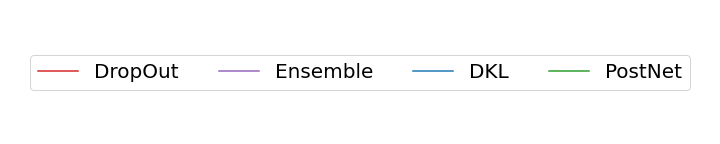
\includegraphics[width=\textwidth]{sections/011_icml2022/resources/legend.png}
    \end{subfigure}
    \vspace{-5mm}
    
    \begin{subfigure}{.245\textwidth}
        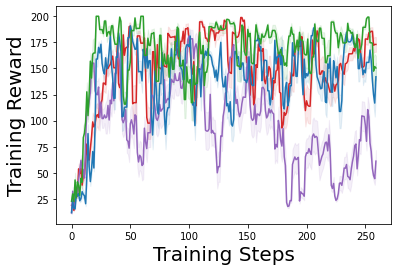
\includegraphics[width=\textwidth]{sections/011_icml2022/resources/cartpole-training_total_reward-training-model.png}
    \end{subfigure}
    \begin{subfigure}{.245\textwidth}
        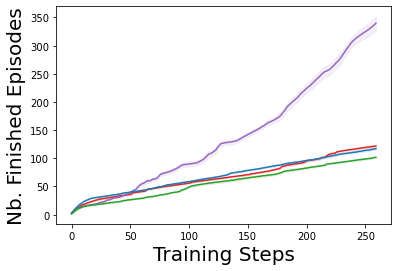
\includegraphics[width=\textwidth]{sections/011_icml2022/resources/cartpole-n_finished_training_episodes-training-model.png}  
    \end{subfigure}
    \begin{subfigure}{.245\textwidth}
        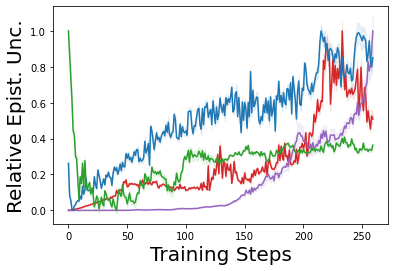
\includegraphics[width=\textwidth]{sections/011_icml2022/resources/cartpole-training_epistemic_uncertainty-training-model.png}
    \end{subfigure}
    \begin{subfigure}{.245\textwidth}
        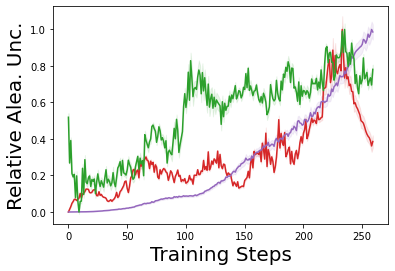
\includegraphics[width=\textwidth]{sections/011_icml2022/resources/cartpole-training_aleatoric_ucertainty-training-model.png}  
    \end{subfigure}
    \caption{Comparison of the training performance of the four uncertainty methods using epsilon-greedy strategies on CartPole. Ideally, a uncertainty aware-model should achieve high reward with few samples and episodes and with a decreasing epistemic uncertainty.}
    \label{fig:model-training-performance-cartpole}
\end{figure}
\begin{figure}
    \centering
        \begin{subfigure}{.5\textwidth}
        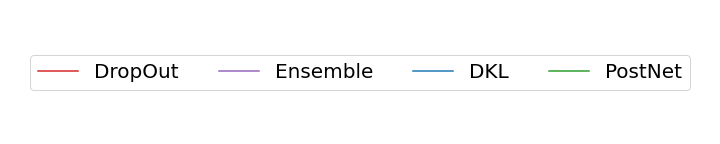
\includegraphics[width=\textwidth]{sections/011_icml2022/resources/legend.png}
    \end{subfigure}
    \vspace{-5mm}
    
    \begin{subfigure}{.245\textwidth}
        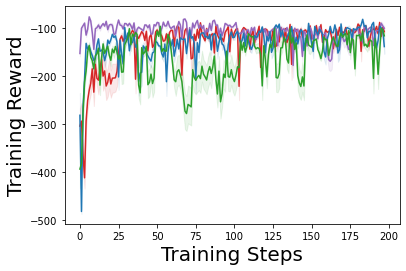
\includegraphics[width=\textwidth]{sections/011_icml2022/resources/acrobot-training_total_reward-training-model.png}
    \end{subfigure}
    \begin{subfigure}{.245\textwidth}
        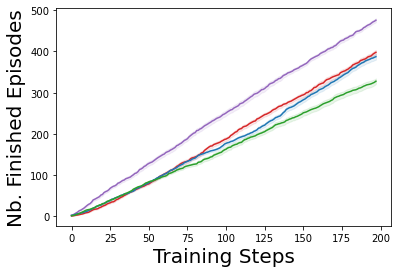
\includegraphics[width=\textwidth]{sections/011_icml2022/resources/acrobot-n_finished_training_episodes-training-model.png}  
    \end{subfigure}
    \begin{subfigure}{.245\textwidth}
        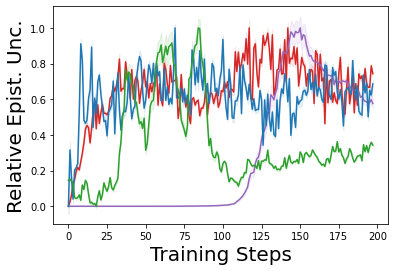
\includegraphics[width=\textwidth]{sections/011_icml2022/resources/acrobot-training_epistemic_uncertainty-training-model.png}
    \end{subfigure}
    \begin{subfigure}{.245\textwidth}
        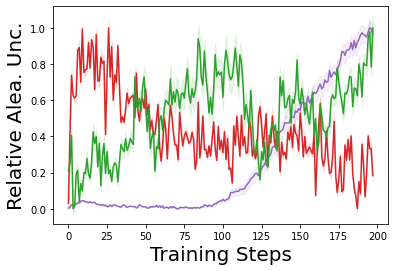
\includegraphics[width=\textwidth]{sections/011_icml2022/resources/acrobot-training_aleatoric_ucertainty-training-model.png}  
    \end{subfigure}
    \caption{Comparison of the training performance of the four uncertainty methods using epsilon-greedy strategies on Acrobot. Ideally, a uncertainty aware-model should achieve high reward with few samples and with a decreasing epistemic uncertainty.}
    \label{fig:model-training-performance-acrobot}
\end{figure}
\begin{figure}
    \centering
        \begin{subfigure}{.5\textwidth}
        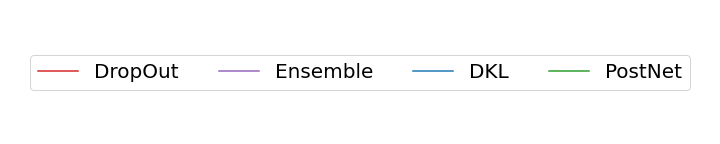
\includegraphics[width=\textwidth]{sections/011_icml2022/resources/legend.png}
    \end{subfigure}
    \vspace{-5mm}
    
    \begin{subfigure}{.245\textwidth}
        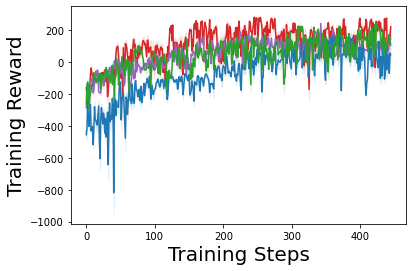
\includegraphics[width=\textwidth]{sections/011_icml2022/resources/lunarlander-training_total_reward-training-model.png}
    \end{subfigure}
    \begin{subfigure}{.245\textwidth}
        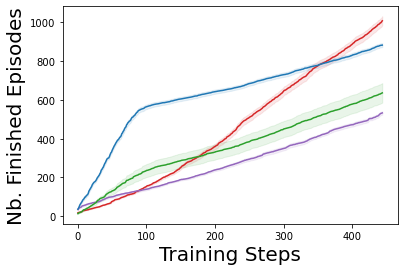
\includegraphics[width=\textwidth]{sections/011_icml2022/resources/lunarlander-n_finished_training_episodes-training-model.png}  
    \end{subfigure}
    \begin{subfigure}{.245\textwidth}
        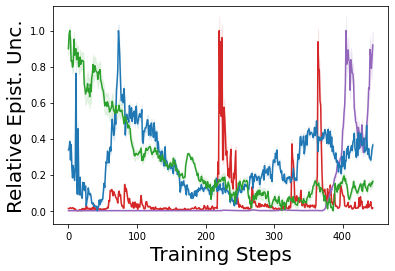
\includegraphics[width=\textwidth]{sections/011_icml2022/resources/lunarlander-training_epistemic_uncertainty-training-model.png}
    \end{subfigure}
    \begin{subfigure}{.245\textwidth}
        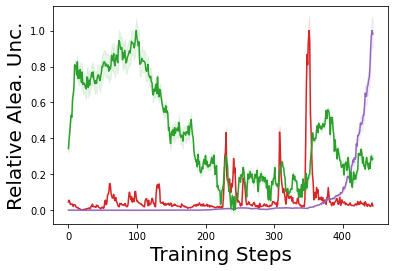
\includegraphics[width=\textwidth]{sections/011_icml2022/resources/lunarlander-training_aleatoric_ucertainty-training-model.png}  
    \end{subfigure}
    \caption{Comparison of the training performance of the four uncertainty methods using epsilon-greedy strategies on LunarLander. Ideally, a uncertainty aware-model should achieve high reward  with few samples and episodes and with a decreasing epistemic uncertainty.}
    \label{fig:model-training-performance-lunarlander}
\end{figure}

We show additional results in fig.~\ref{fig:strategy-training-performance-cartpole}, fig.~\ref{fig:strategy-training-performance-acrobot} and fig.~\ref{fig:strategy-training-performance-lunarlander} to compare the performance of the sampling-epistemic and the sampling-aleatoric strategies at training time. The sampling-epistemic strategy consistently achieve a better sample efficiency. Thus, Ensemble, DropOut and PostNet empirically satisfy des.~\ref{ax:training_strategy}. Hence, disentangling aleatoric and epistemic uncertainty can speed learning in a training environment.

\begin{figure}
    \centering
    \begin{subfigure}{.45\textwidth}
        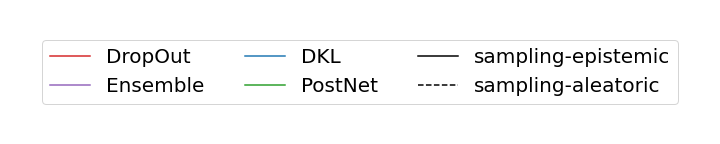
\includegraphics[width=\textwidth]{sections/011_icml2022/resources/sampling-legend.png}
    \end{subfigure}
    \vspace{-3mm}
    
    \begin{subfigure}{.245\textwidth}
        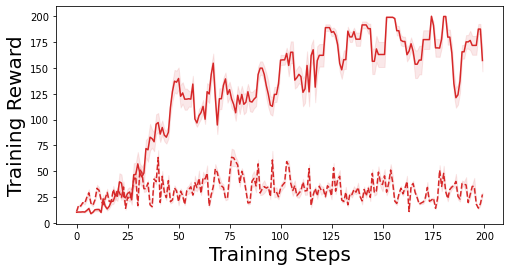
\includegraphics[width=\textwidth]{sections/011_icml2022/resources/cartpole-training_total_reward-dropout-training-strategy.png}
    \end{subfigure}
    \begin{subfigure}{.245\textwidth}
        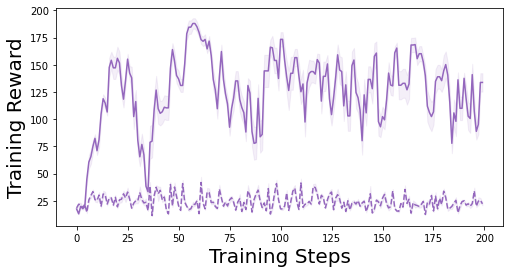
\includegraphics[width=\textwidth]{sections/011_icml2022/resources/cartpole-training_total_reward-ensemble-training-strategy.png}
    \end{subfigure}
    \begin{subfigure}{.245\textwidth}
        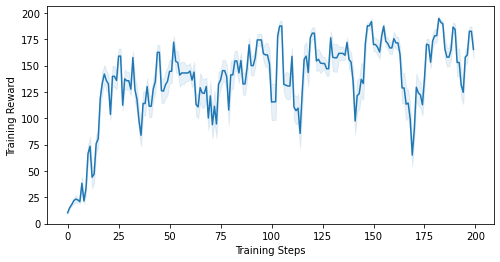
\includegraphics[width=\textwidth]{sections/011_icml2022/resources/cartpole-training_total_reward-dkl-training-strategy.png}
    \end{subfigure}
    \begin{subfigure}{.245\textwidth}
        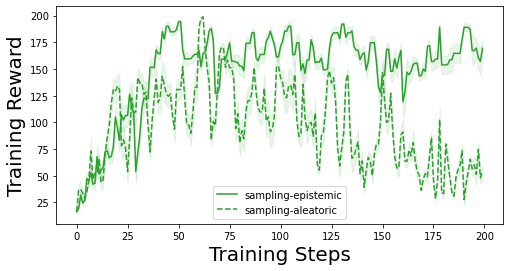
\includegraphics[width=\textwidth]{sections/011_icml2022/resources/cartpole-training_total_reward-postnet-training-strategy.png}
    \end{subfigure}
    
    \begin{subfigure}{.245\textwidth}
        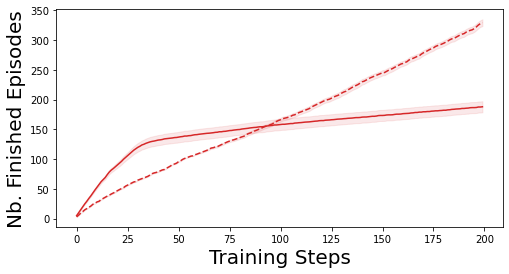
\includegraphics[width=\textwidth]{sections/011_icml2022/resources/cartpole-n_finished_training_episodes-dropout-training-strategy.png}
    \end{subfigure}
    \begin{subfigure}{.245\textwidth}
        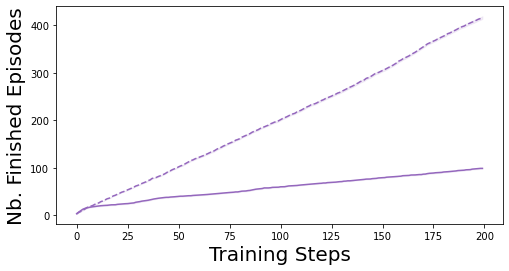
\includegraphics[width=\textwidth]{sections/011_icml2022/resources/cartpole-n_finished_training_episodes-ensemble-training-strategy.png}
    \end{subfigure}
    \begin{subfigure}{.245\textwidth}
        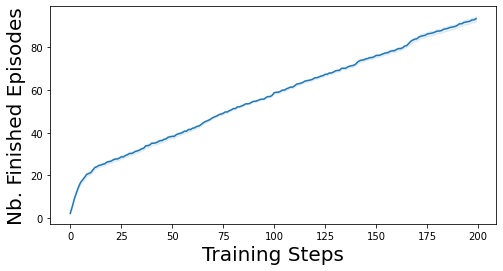
\includegraphics[width=\textwidth]{sections/011_icml2022/resources/cartpole-n_finished_training_episodes-dkl-training-strategy.png}
    \end{subfigure}
    \begin{subfigure}{.245\textwidth}
        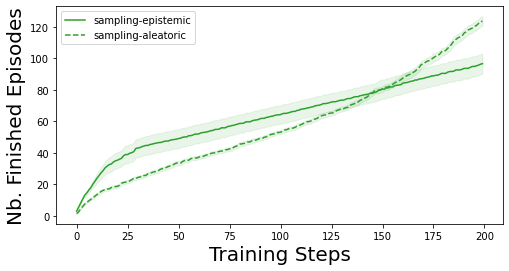
\includegraphics[width=\textwidth]{sections/011_icml2022/resources/cartpole-n_finished_training_episodes-postnet-training-strategy.png}
    \end{subfigure}
    \caption{Comparison of the training performance on Cartpole. The four uncertainty methods use the sampling-aleatoric or the sampling-epistemic at training time. Ideally, an uncertainty aware-model should high reward with few samples.}
    \label{fig:strategy-training-performance-cartpole}
\end{figure}
\begin{figure}
    \centering
    \begin{subfigure}{.45\textwidth}
        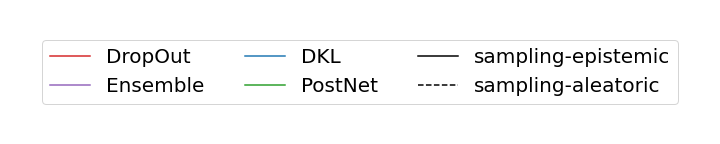
\includegraphics[width=\textwidth]{sections/011_icml2022/resources/sampling-legend.png}
    \end{subfigure}
    \vspace{-3mm}
    
    \begin{subfigure}{.245\textwidth}
        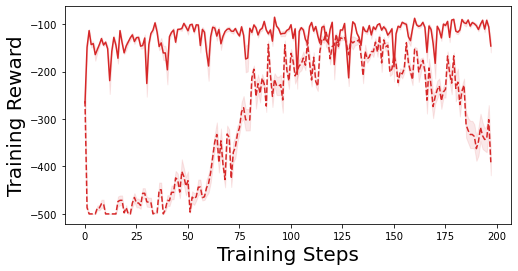
\includegraphics[width=\textwidth]{sections/011_icml2022/resources/acrobot-training_total_reward-dropout-training-strategy.png}
    \end{subfigure}
    \begin{subfigure}{.245\textwidth}
        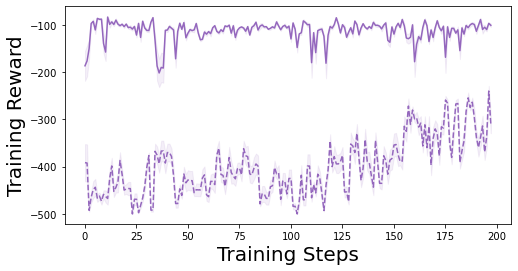
\includegraphics[width=\textwidth]{sections/011_icml2022/resources/acrobot-training_total_reward-ensemble-training-strategy.png}
    \end{subfigure}
    \begin{subfigure}{.245\textwidth}
        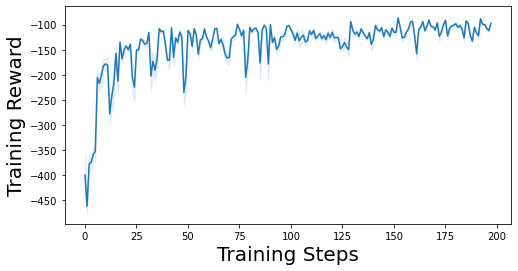
\includegraphics[width=\textwidth]{sections/011_icml2022/resources/acrobot-training_total_reward-dkl-training-strategy.png}
    \end{subfigure}
    \begin{subfigure}{.245\textwidth}
        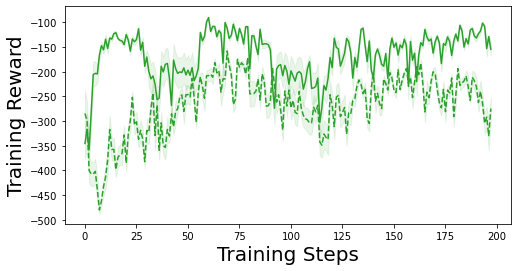
\includegraphics[width=\textwidth]{sections/011_icml2022/resources/acrobot-training_total_reward-postnet-training-strategy.png}
    \end{subfigure}
    
    \begin{subfigure}{.245\textwidth}
        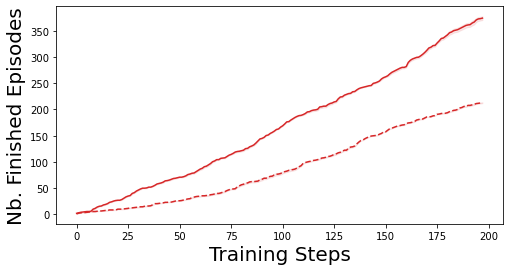
\includegraphics[width=\textwidth]{sections/011_icml2022/resources/acrobot-n_finished_training_episodes-dropout-training-strategy.png}
    \end{subfigure}
    \begin{subfigure}{.245\textwidth}
        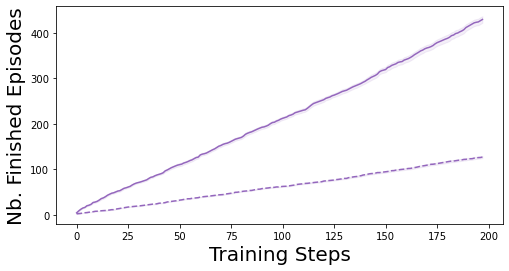
\includegraphics[width=\textwidth]{sections/011_icml2022/resources/acrobot-n_finished_training_episodes-ensemble-training-strategy.png}
    \end{subfigure}
    \begin{subfigure}{.245\textwidth}
        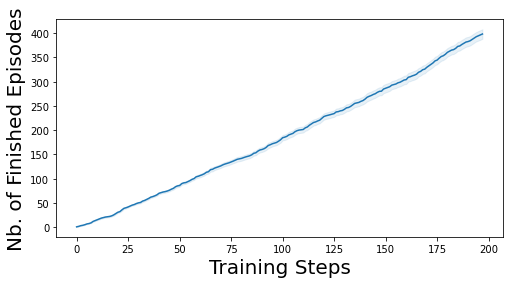
\includegraphics[width=\textwidth]{sections/011_icml2022/resources/acrobot-n_finished_training_episodes-dkl-training-strategy.png}
    \end{subfigure}
    \begin{subfigure}{.245\textwidth}
        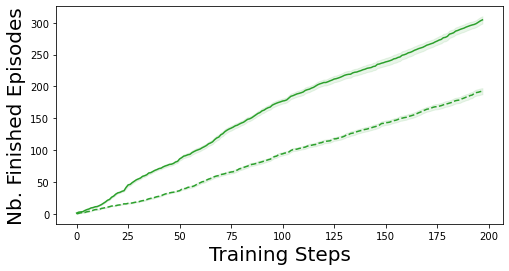
\includegraphics[width=\textwidth]{sections/011_icml2022/resources/acrobot-n_finished_training_episodes-postnet-training-strategy.png}
    \end{subfigure}
    \caption{Comparison of the training performance on Acrobot. The four uncertainty methods use the sampling-aleatoric or the sampling-epistemic at training time. Ideally, an uncertainty aware-model should high reward with few samples.}
    \label{fig:strategy-training-performance-acrobot}
\end{figure}
\begin{figure}
    \centering
    \begin{subfigure}{.45\textwidth}
        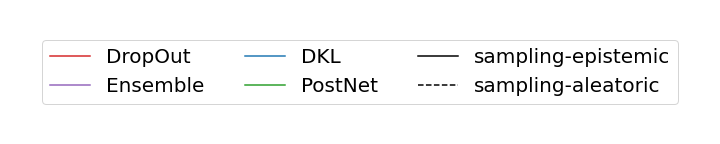
\includegraphics[width=\textwidth]{sections/011_icml2022/resources/sampling-legend.png}
    \end{subfigure}
    \vspace{-3mm}
    
    \begin{subfigure}{.245\textwidth}
        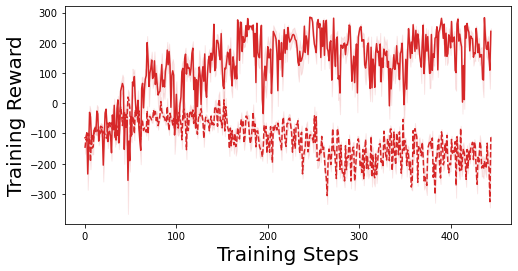
\includegraphics[width=\textwidth]{sections/011_icml2022/resources/lunarlander-training_total_reward-dropout-training-strategy.png}
    \end{subfigure}
    \begin{subfigure}{.245\textwidth}
        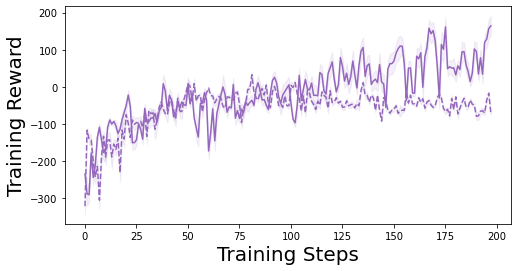
\includegraphics[width=\textwidth]{sections/011_icml2022/resources/lunarlander-training_total_reward-ensemble-training-strategy.png}
    \end{subfigure}
    \begin{subfigure}{.245\textwidth}
        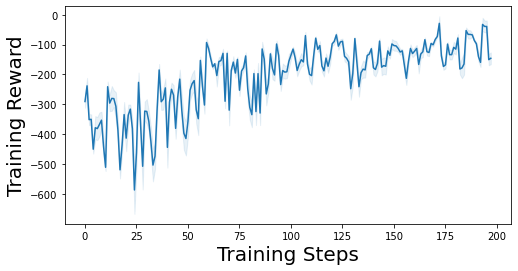
\includegraphics[width=\textwidth]{sections/011_icml2022/resources/lunarlander-training_total_reward-dkl-training-strategy.png}
    \end{subfigure}
    \begin{subfigure}{.245\textwidth}
        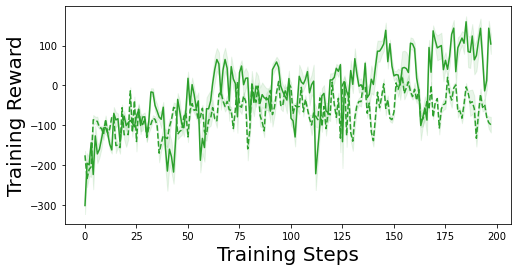
\includegraphics[width=\textwidth]{sections/011_icml2022/resources/lunarlander-training_total_reward-postnet-training-strategy.png}
    \end{subfigure}
    
    \begin{subfigure}{.245\textwidth}
        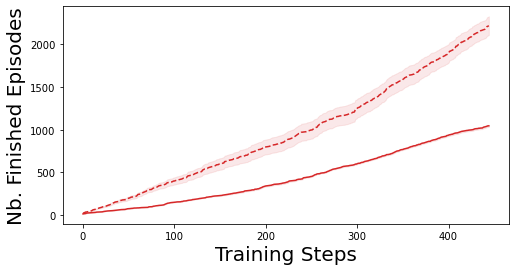
\includegraphics[width=\textwidth]{sections/011_icml2022/resources/lunarlander-n_finished_training_episodes-dropout-training-strategy.png}
    \end{subfigure}
    \begin{subfigure}{.245\textwidth}
        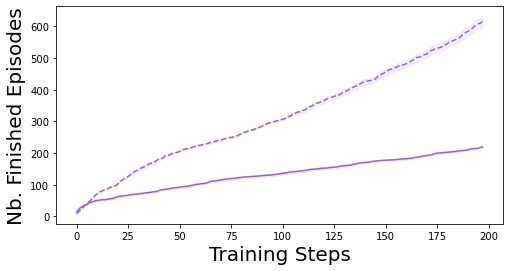
\includegraphics[width=\textwidth]{sections/011_icml2022/resources/lunarlander-n_finished_training_episodes-ensemble-training-strategy.png}
    \end{subfigure}
    \begin{subfigure}{.245\textwidth}
        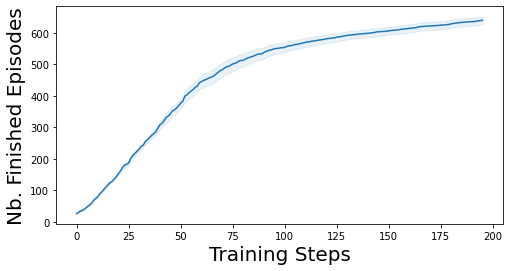
\includegraphics[width=\textwidth]{sections/011_icml2022/resources/lunarlander-n_finished_training_episodes-dkl-training-strategy.png}
    \end{subfigure}
    \begin{subfigure}{.245\textwidth}
        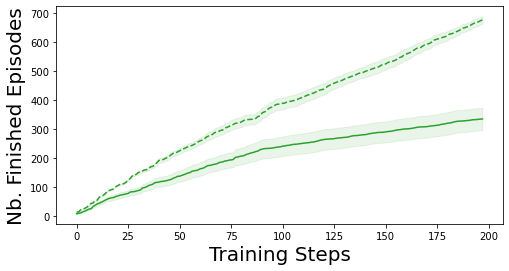
\includegraphics[width=\textwidth]{sections/011_icml2022/resources/lunarlander-n_finished_training_episodes-postnet-training-strategy.png}
    \end{subfigure}
    \caption{Comparison of the training performance on LunarLander. The four uncertainty methods use the sampling-aleatoric or the sampling-epistemic at training time. Ideally, an uncertainty aware-model should high reward with few samples.}
    \label{fig:strategy-training-performance-lunarlander}
\end{figure}

\subsection{Testing Time}

We show additional results in fig.~\ref{fig:model-testing-performance-cartpole}, fig.~\ref{fig:model-testing-performance-acrobot} and fig.~\ref{fig:model-testing-performance-lunarlander} to compare the generalization and OOD detection performance of the uncertainty estimates of the four uncertainty methods at testing time. The models use the sampling-epistemic or the sampling-aleatoric strategy at both training and testing time. Further, we show other additional results for OOD detection by using the area under the precision-recall (AUC-PR) scores instead of the area under the receiver operating characteristic curve (AUC-ROC) in fig.~\ref{fig:strategy-testing-ood-auc-pr-performance-cartpole}, fig.~\ref{fig:strategy-testing-ood-auc-pr-performance-acrobot}, fig.~\ref{fig:strategy-testing-ood-auc-pr-performance-lunarlander}. We observe that DKL and PostNet achieve  very high OOD detection scores in most settings  compared to DropOut and Ensemble. These \emph{empirical} results align with the \emph{theoretical} results stating that DKL and PostNet should assign high uncertainty to states very different from states observed during training. Thus, DKL and PostNet validate des.~\ref{ax:testing_state}. In particular, DKL and PostNet can reliably equip DQN with epistemic uncertainty estimates which can be used to flag anomalous OOD states.

\begin{figure}
    \centering
    \vspace{-7mm}
        \begin{subfigure}{.5\textwidth}
        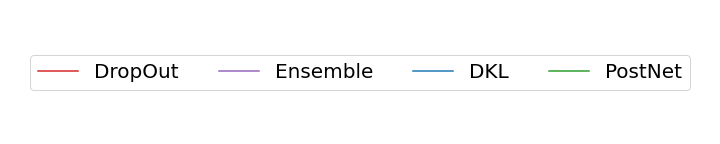
\includegraphics[width=\textwidth]{sections/011_icml2022/resources/legend.png}
    \end{subfigure}
    \vspace{-5mm}
    
    \begin{subfigure}{.4\textwidth}
        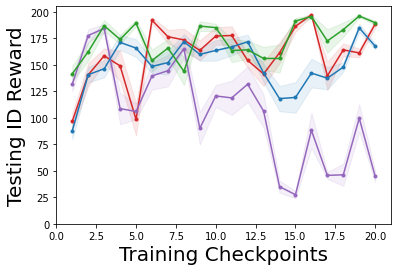
\includegraphics[width=\textwidth]{sections/011_icml2022/resources/CartPole-v0-mean_reward_-testing-model.png}  
    \end{subfigure}
    \begin{subfigure}{.4\textwidth}
        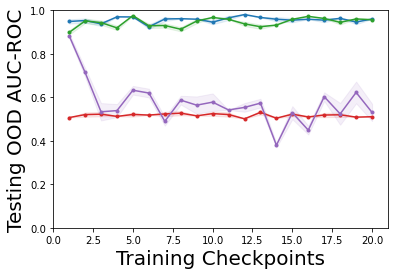
\includegraphics[width=\textwidth]{sections/011_icml2022/resources/CartPoleOOD-v0-AUC-ROC-epistemic_-testing-model.png}
    \end{subfigure}
        \vspace{-3mm}
    \caption{Comparison of the testing performance of the four uncertainty methods using epsilon-greedy strategies at training and testing time on CartPole. Ideally, an uncertainty aware-model should achieve high reward and high OOD detection scores.}
    \label{fig:model-testing-performance-cartpole}
    \vspace{-4mm}
\end{figure}
\begin{figure}
    \centering
        \begin{subfigure}{.5\textwidth}
        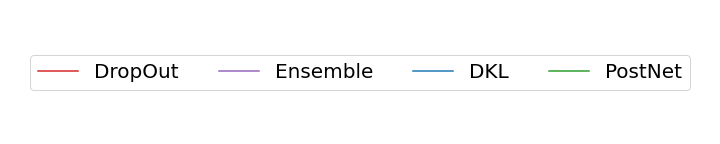
\includegraphics[width=\textwidth]{sections/011_icml2022/resources/legend.png}
    \end{subfigure}
    \vspace{-5mm}
    
    \begin{subfigure}{.4\textwidth}
        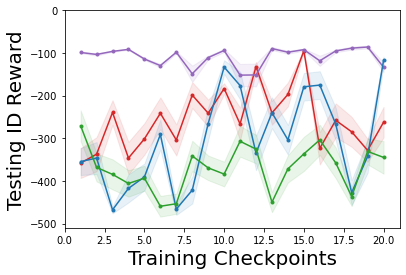
\includegraphics[width=\textwidth]{sections/011_icml2022/resources/Acrobot-v1-mean_reward_-testing-model.png}  
    \end{subfigure}
    \begin{subfigure}{.4\textwidth}
        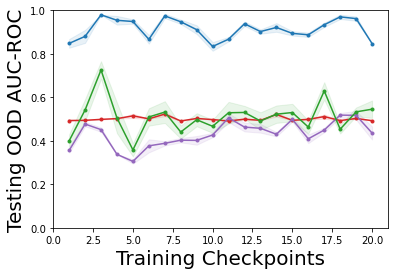
\includegraphics[width=\textwidth]{sections/011_icml2022/resources/AcrobotOOD-v0-AUC-ROC-epistemic_-testing-model.png}
    \end{subfigure}
    \caption{Comparison of the testing performance of the four uncertainty methods using epsilon-greedy strategies at training and testing time on Acrobot. Ideally, an uncertainty aware-model should achieve high reward and high OOD detection scores.}
    \label{fig:model-testing-performance-acrobot}
\end{figure}
\begin{figure}
    \centering
        \begin{subfigure}{.5\textwidth}
        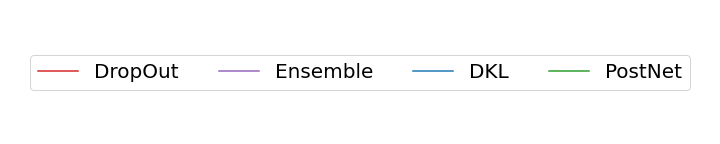
\includegraphics[width=\textwidth]{sections/011_icml2022/resources/legend.png}
    \end{subfigure}
    \vspace{-5mm}
    
    \begin{subfigure}{.4\textwidth}
        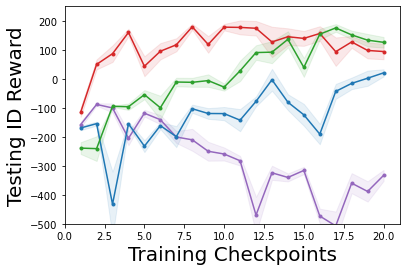
\includegraphics[width=\textwidth]{sections/011_icml2022/resources/LunarLander-v2-mean_reward_-testing-model.png}  
    \end{subfigure}
    \begin{subfigure}{.4\textwidth}
        \includegraphics[width=\textwidth]{sections/011_icml2022/resources/LunarLanderOOD-v0-AUC-ROC-epistemic_-testing-model.png}
    \end{subfigure}
    \caption{Comparison of the testing performance of the four uncertainty methods using epsilon-greedy strategies at training and testing time on LunarLander. Ideally, an uncertainty aware-model should achieve high reward and high OOD detection scores.}
    \label{fig:model-testing-performance-lunarlander}
\end{figure}

We show additional results in fig.~\ref{fig:strategy-testing-performance-cartpole}, fig.~\ref{fig:strategy-testing-performance-acrobot} and fig.~\ref{fig:strategy-testing-performance-lunarlander} to compare the performance of the sampling-epistemic and sampling-aleatoric strategies for each uncertainty model. All models use the same epsilon-greedy strategy at training time. We observe that the sampling-epistemic strategy is consistently better than sampling-aleatoric at testing time. The higher generalization capacity of the sampling-epistemic strategy aligns with \cite{epistemic-pomdp} which recasts the problem of generalization in RL as solving an epistemic POMDP. These empirical results underline the need to disentangle both aleatoric and epistemic uncertainty for high reward performance at testing time.

\begin{figure}
    \centering
    \begin{subfigure}{.45\textwidth}
        \includegraphics[width=\textwidth]{sections/011_icml2022/resources/sampling-legend.png}
    \end{subfigure}
    \vspace{-3mm}
    
    \begin{subfigure}{.245\textwidth}
        \includegraphics[width=\textwidth]{sections/011_icml2022/resources/DropOut-CartPole-v0-mean_reward_-testing-strategy.png}
    \end{subfigure}
    \begin{subfigure}{.245\textwidth}
        \includegraphics[width=\textwidth]{sections/011_icml2022/resources/Ensemble-CartPole-v0-mean_reward_-testing-strategy.png}
    \end{subfigure}
    \begin{subfigure}{.245\textwidth}
        \includegraphics[width=\textwidth]{sections/011_icml2022/resources/DKL-CartPole-v0-mean_reward_-testing-strategy.png}
    \end{subfigure}
    \begin{subfigure}{.245\textwidth}
        \includegraphics[width=\textwidth]{sections/011_icml2022/resources/PostNet-CartPole-v0-mean_reward_-testing-strategy.png}
    \end{subfigure}
    
    \begin{subfigure}{.245\textwidth}
        \includegraphics[width=\textwidth]{sections/011_icml2022/resources/DropOut-CartPoleOOD-v0-AUC-ROC-epistemic_-testing-strategy.png}
    \end{subfigure}
    \begin{subfigure}{.245\textwidth}
        \includegraphics[width=\textwidth]{sections/011_icml2022/resources/Ensemble-CartPoleOOD-v0-AUC-ROC-epistemic_-testing-strategy.png}
    \end{subfigure}
    \begin{subfigure}{.245\textwidth}
        \includegraphics[width=\textwidth]{sections/011_icml2022/resources/DKL-CartPoleOOD-v0-AUC-ROC-epistemic_-testing-strategy.png}
    \end{subfigure}
    \begin{subfigure}{.245\textwidth}
        \includegraphics[width=\textwidth]{sections/011_icml2022/resources/PostNet-CartPoleOOD-v0-AUC-ROC-epistemic_-testing-strategy.png}
    \end{subfigure}
    \caption{Comparison of the testing reward and OOD performance on CartPole. The four uncertainty methods use the sampling-aleatoric or sampling-epistemic strategies at both training and testing time. Ideally, an uncertainty aware-model should achieve high testing reward and high OOD AUC-ROC detection score.}
    \label{fig:strategy-testing-performance-cartpole}
\end{figure}
\begin{figure}
    \centering
    \begin{subfigure}{.45\textwidth}
        \includegraphics[width=\textwidth]{sections/011_icml2022/resources/sampling-legend.png}
    \end{subfigure}
    \vspace{-3mm}
    
    \begin{subfigure}{.245\textwidth}
        \includegraphics[width=\textwidth]{sections/011_icml2022/resources/DropOut-Acrobot-v1-mean_reward_-testing-strategy.png}
    \end{subfigure}
    \begin{subfigure}{.245\textwidth}
        \includegraphics[width=\textwidth]{sections/011_icml2022/resources/Ensemble-Acrobot-v1-mean_reward_-testing-strategy.png}
    \end{subfigure}
    \begin{subfigure}{.245\textwidth}
        \includegraphics[width=\textwidth]{sections/011_icml2022/resources/DKL-Acrobot-v1-mean_reward_-testing-strategy.png}
    \end{subfigure}
    \begin{subfigure}{.245\textwidth}
        \includegraphics[width=\textwidth]{sections/011_icml2022/resources/PostNet-Acrobot-v1-mean_reward_-testing-strategy.png}
    \end{subfigure}
    
    \begin{subfigure}{.245\textwidth}
        \includegraphics[width=\textwidth]{sections/011_icml2022/resources/DropOut-AcrobotOOD-v0-AUC-ROC-epistemic_-testing-strategy.png}
    \end{subfigure}
    \begin{subfigure}{.245\textwidth}
        \includegraphics[width=\textwidth]{sections/011_icml2022/resources/Ensemble-AcrobotOOD-v0-AUC-ROC-epistemic_-testing-strategy.png}
    \end{subfigure}
    \begin{subfigure}{.245\textwidth}
        \includegraphics[width=\textwidth]{sections/011_icml2022/resources/DKL-AcrobotOOD-v0-AUC-ROC-epistemic_-testing-strategy.png}
    \end{subfigure}
    \begin{subfigure}{.245\textwidth}
        \includegraphics[width=\textwidth]{sections/011_icml2022/resources/PostNet-AcrobotOOD-v0-AUC-ROC-epistemic_-testing-strategy.png}
    \end{subfigure}
    \caption{Comparison of the testing reward and OOD performance on Acrobot. The four uncertainty methods use the sampling-aleatoric or sampling-epistemic strategies at both training and testing time. Ideally, an uncertainty aware-model should achieve high testing reward and high OOD AUC-ROC detection score.}
    \label{fig:strategy-testing-performance-acrobot}
\end{figure}
%\begin{figure*}
    \centering
        % \vspace{-6mm}
    \begin{subfigure}{.45\textwidth}
        \includegraphics[width=\textwidth]{sections/011_icml2022/resources/sampling-legend.png}
    \end{subfigure}
    \vspace{-5mm}
    
    \begin{subfigure}{.2\textwidth}
        \includegraphics[width=\textwidth]{sections/011_icml2022/resources/DropOut-LunarLander-v2-mean_reward_-testing-strategy.png}
    \end{subfigure}
    \begin{subfigure}{.2\textwidth}
        \includegraphics[width=\textwidth]{sections/011_icml2022/resources/Ensemble-LunarLander-v2-mean_reward_-testing-strategy.png}
    \end{subfigure}
    \begin{subfigure}{.2\textwidth}
        \includegraphics[width=\textwidth]{sections/011_icml2022/resources/DKL-LunarLander-v2-mean_reward_-testing-strategy.png}
    \end{subfigure}
    \begin{subfigure}{.2\textwidth}
        \includegraphics[width=\textwidth]{sections/011_icml2022/resources/PostNet-LunarLander-v2-mean_reward_-testing-strategy.png}
    \end{subfigure}
    
    \begin{subfigure}{.2\textwidth}
        \includegraphics[width=\textwidth]{sections/011_icml2022/resources/DropOut-LunarLanderOOD-v0-AUC-ROC-epistemic_-testing-strategy.png}
    \end{subfigure}
    \begin{subfigure}{.2\textwidth}
        \includegraphics[width=\textwidth]{sections/011_icml2022/resources/Ensemble-LunarLanderOOD-v0-AUC-ROC-epistemic_-testing-strategy.png}
    \end{subfigure}
    \begin{subfigure}{.2\textwidth}
        \includegraphics[width=\textwidth]{sections/011_icml2022/resources/DKL-LunarLanderOOD-v0-AUC-ROC-epistemic_-testing-strategy.png}
    \end{subfigure}
    \begin{subfigure}{.2\textwidth}
        \includegraphics[width=\textwidth]{sections/011_icml2022/resources/PostNet-LunarLanderOOD-v0-AUC-ROC-epistemic_-testing-strategy.png}
    \end{subfigure}
        % \vspace{-3mm}
    \caption{Comparison of the testing reward and OOD performance on LunarLander. The four uncertainty methods use the sampling-aleatoric or sampling-epistemic strategies at both training and testing time. Ideally, an uncertainty aware-model should achieve high testing reward and high OOD AUC-ROC detection score.}
    \label{fig:strategy-testing-performance-lunarlander}
        % \vspace{-6mm}
\end{figure*}

We show additional results in fig.~\ref{fig:strategy-state-shift-testing-performance-cartpole}, fig.~\ref{fig:strategy-state-shift-testing-performance-acrobot}, fig.~\ref{fig:strategy-state-shift-testing-performance-lunarlander}, fig.~\ref{fig:strategy-action-shift-testing-performance-cartpole}, fig.~\ref{fig:strategy-action-shift-testing-performance-acrobot}, fig.~\ref{fig:strategy-action-shift-testing-performance-lunarlander}, fig.~\ref{fig:strategy-transition-shift-testing-performance-cartpole}, fig.~\ref{fig:strategy-transition-shift-testing-performance-acrobot}, fig.~\ref{fig:strategy-transition-shift-testing-performance-lunarlander} to compare the generalization and uncertainty performances of the sampling-epistemic and sampling-aleatoric strategies of each method on perturbed environments with state, action and transition dynamic perturbations. All methods achieve lower reward on environment with stronger perturbations. This is expected since a model cannot generalize to all new environments. The sampling-epistemic strategy achieves significantly better that the sampling-aleatoric strategy. The generalization capacity of the sampling-epistemic strategy aligns again with \cite{epistemic-pomdp}. Thus, differentiating between aleatoric and epistemic uncertainty can improve generalization. Finally, only DKL and PostNet reliably assign higher epistemic uncertainty to most of the perturbation types. Therefore, DKL and PostNet have a good trade-off between generalization and detection of new perturbed environments.

\textbf{Video:} For a better visualization, we attach supplementary videos showing the landing performance, the reward performance, and the relatice epistemic uncertainty prediction of the PostNet model in the original LunarLander environments and two environments with perturbed states with perturbation strengths equal to $0.5$ and $2.0$. On the original environment, we observe that the space ship lands correctly with lower epistemic uncertainty after landing. On the perturbed environment with strength $0.5$, we observe that the space ship avoids crashing but assigns higher epistemic uncertainty when moving further from the landing zone. Finally, on the perturbed environment with strength $2.0$, we observe that the space ship assigns significantly higher epistemic uncertainty especially when approaching the floor before the crash.

\begin{figure*}
    \centering
        \vspace{-6mm}
    \begin{subfigure}{.45\textwidth}
        \includegraphics[width=\textwidth]{sections/011_icml2022/resources/sampling-legend.png}
    \end{subfigure}
    \vspace{-3mm}
    
    \begin{subfigure}{.24\textwidth}
        \includegraphics[width=\textwidth]{sections/011_icml2022/resources/state_shift-DropOut-CartPoleShift-v0-mean_reward_.png}
    \end{subfigure}
    \begin{subfigure}{.24\textwidth}
        \includegraphics[width=\textwidth]{sections/011_icml2022/resources/state_shift-Ensemble-CartPoleShift-v0-mean_reward_.png}
    \end{subfigure}
    \begin{subfigure}{.24\textwidth}
        \includegraphics[width=\textwidth]{sections/011_icml2022/resources/state_shift-DKL-CartPoleShift-v0-mean_reward_.png}
    \end{subfigure}
    \begin{subfigure}{.24\textwidth}
        \includegraphics[width=\textwidth]{sections/011_icml2022/resources/state_shift-PostNet-CartPoleShift-v0-mean_reward_.png}
    \end{subfigure}
    
    \begin{subfigure}{.24\textwidth}
        \includegraphics[width=\textwidth]{sections/011_icml2022/resources/state_shift-DropOut-CartPoleShift-v0-mean_epistemic_uncertainty_.png}
    \end{subfigure}
    \begin{subfigure}{.24\textwidth}
        \includegraphics[width=\textwidth]{sections/011_icml2022/resources/state_shift-Ensemble-CartPoleShift-v0-mean_epistemic_uncertainty_.png}
    \end{subfigure}
    \begin{subfigure}{.24\textwidth}
        \includegraphics[width=\textwidth]{sections/011_icml2022/resources/state_shift-DKL-CartPoleShift-v0-mean_epistemic_uncertainty_.png}
    \end{subfigure}
    \begin{subfigure}{.24\textwidth}
        \includegraphics[width=\textwidth]{sections/011_icml2022/resources/state_shift-PostNet-CartPoleShift-v0-mean_epistemic_uncertainty_.png}
    \end{subfigure}
        \vspace{-2mm}
    \caption{Comparison of the testing performance and the epistemic uncertainty predictions on CartPole with perturbed states. The four uncertainty methods use the epsilon-greedy strategy at training time and the sampling-aleatoric or sampling-epistemic strategy at testing time. Ideally, an uncertainty-aware model should maintain high reward while assigning higher epistemic uncertainty on more severe perturbations.}
    \label{fig:strategy-state-shift-testing-performance-cartpole}
        \vspace{-6mm}
\end{figure*}
\begin{figure}
    \centering
    \begin{subfigure}{.45\textwidth}
        \includegraphics[width=\textwidth]{sections/011_icml2022/resources/sampling-legend.png}
    \end{subfigure}
    \vspace{-3mm}
    
    \begin{subfigure}{.245\textwidth}
        \includegraphics[width=\textwidth]{sections/011_icml2022/resources/action_shift-DropOut-CartPoleShift-v0-mean_reward_.png}
    \end{subfigure}
    \begin{subfigure}{.245\textwidth}
        \includegraphics[width=\textwidth]{sections/011_icml2022/resources/action_shift-Ensemble-CartPoleShift-v0-mean_reward_.png}
    \end{subfigure}
    \begin{subfigure}{.245\textwidth}
        \includegraphics[width=\textwidth]{sections/011_icml2022/resources/action_shift-DKL-CartPoleShift-v0-mean_reward_.png}
    \end{subfigure}
    \begin{subfigure}{.245\textwidth}
        \includegraphics[width=\textwidth]{sections/011_icml2022/resources/action_shift-PostNet-CartPoleShift-v0-mean_reward_.png}
    \end{subfigure}
    
    \begin{subfigure}{.245\textwidth}
        \includegraphics[width=\textwidth]{sections/011_icml2022/resources/action_shift-DropOut-CartPoleShift-v0-mean_epistemic_uncertainty_.png}
    \end{subfigure}
    \begin{subfigure}{.245\textwidth}
        \includegraphics[width=\textwidth]{sections/011_icml2022/resources/action_shift-Ensemble-CartPoleShift-v0-mean_epistemic_uncertainty_.png}
    \end{subfigure}
    \begin{subfigure}{.245\textwidth}
        \includegraphics[width=\textwidth]{sections/011_icml2022/resources/action_shift-DKL-CartPoleShift-v0-mean_epistemic_uncertainty_.png}
    \end{subfigure}
    \begin{subfigure}{.245\textwidth}
        \includegraphics[width=\textwidth]{sections/011_icml2022/resources/action_shift-PostNet-CartPoleShift-v0-mean_epistemic_uncertainty_.png}
    \end{subfigure}
    \caption{Comparison of the testing performance and the epistemic uncertainty predictions on CartPole with perturbed actions. The four uncertainty methods use the epsilon-greedy strategy at training time and the sampling-aleatoric or sampling-epistemic strategy at testing time. Ideally, an uncertainty-aware model should maintain high reward while assigning higher epistemic uncertainty on more severe perturbations.}
    \label{fig:strategy-action-shift-testing-performance-cartpole}
\end{figure}
\begin{figure}
    \centering
        \vspace{-3mm}
    \begin{subfigure}{.45\textwidth}
        \includegraphics[width=\textwidth]{sections/011_icml2022/resources/sampling-legend.png}
    \end{subfigure}
    \vspace{-3mm}
    
    \begin{subfigure}{.245\textwidth}
        \includegraphics[width=\textwidth]{sections/011_icml2022/resources/transition_shift-DropOut-CartPoleShift-v0-mean_reward_.png}
    \end{subfigure}
    \begin{subfigure}{.245\textwidth}
        \includegraphics[width=\textwidth]{sections/011_icml2022/resources/transition_shift-Ensemble-CartPoleShift-v0-mean_reward_.png}
    \end{subfigure}
    \begin{subfigure}{.245\textwidth}
        \includegraphics[width=\textwidth]{sections/011_icml2022/resources/transition_shift-DKL-CartPoleShift-v0-mean_reward_.png}
    \end{subfigure}
    \begin{subfigure}{.245\textwidth}
        \includegraphics[width=\textwidth]{sections/011_icml2022/resources/transition_shift-PostNet-CartPoleShift-v0-mean_reward_.png}
    \end{subfigure}
    
    \begin{subfigure}{.245\textwidth}
        \includegraphics[width=\textwidth]{sections/011_icml2022/resources/transition_shift-DropOut-CartPoleShift-v0-mean_epistemic_uncertainty_.png}
    \end{subfigure}
    \begin{subfigure}{.245\textwidth}
        \includegraphics[width=\textwidth]{sections/011_icml2022/resources/transition_shift-Ensemble-CartPoleShift-v0-mean_epistemic_uncertainty_.png}
    \end{subfigure}
    \begin{subfigure}{.245\textwidth}
        \includegraphics[width=\textwidth]{sections/011_icml2022/resources/transition_shift-DKL-CartPoleShift-v0-mean_epistemic_uncertainty_.png}
    \end{subfigure}
    \begin{subfigure}{.245\textwidth}
        \includegraphics[width=\textwidth]{sections/011_icml2022/resources/transition_shift-PostNet-CartPoleShift-v0-mean_epistemic_uncertainty_.png}
    \end{subfigure}
        \vspace{-2mm}
    \caption{Comparison of the testing performance and the epistemic uncertainty predictions on CartPole with perturbed transitions. The four uncertainty methods use the epsilon-greedy strategy at training time and the sampling-aleatoric or sampling-epistemic strategy at testing time. Ideally, an uncertainty-aware model should maintain high reward while assigning higher epistemic uncertainty on more severe perturbations.}
    \label{fig:strategy-transition-shift-testing-performance-cartpole}
        \vspace{-3mm}
\end{figure}
\begin{figure}
    \centering
        \vspace{-6mm}
    \begin{subfigure}{.45\textwidth}
        \includegraphics[width=\textwidth]{sections/011_icml2022/resources/sampling-legend.png}
    \end{subfigure}
    \vspace{-3mm}
    
    \begin{subfigure}{.245\textwidth}
        \includegraphics[width=\textwidth]{sections/011_icml2022/resources/state_shift-DropOut-AcrobotShift-v0-mean_reward_.png}
    \end{subfigure}
    \begin{subfigure}{.245\textwidth}
        \includegraphics[width=\textwidth]{sections/011_icml2022/resources/state_shift-Ensemble-AcrobotShift-v0-mean_reward_.png}
    \end{subfigure}
    \begin{subfigure}{.245\textwidth}
        \includegraphics[width=\textwidth]{sections/011_icml2022/resources/state_shift-DKL-AcrobotShift-v0-mean_reward_.png}
    \end{subfigure}
    \begin{subfigure}{.245\textwidth}
        \includegraphics[width=\textwidth]{sections/011_icml2022/resources/state_shift-PostNet-AcrobotShift-v0-mean_reward_.png}
    \end{subfigure}
    
    \begin{subfigure}{.245\textwidth}
        \includegraphics[width=\textwidth]{sections/011_icml2022/resources/state_shift-DropOut-AcrobotShift-v0-mean_epistemic_uncertainty_.png}
    \end{subfigure}
    \begin{subfigure}{.245\textwidth}
        \includegraphics[width=\textwidth]{sections/011_icml2022/resources/state_shift-Ensemble-AcrobotShift-v0-mean_epistemic_uncertainty_.png}
    \end{subfigure}
    \begin{subfigure}{.245\textwidth}
        \includegraphics[width=\textwidth]{sections/011_icml2022/resources/state_shift-DKL-AcrobotShift-v0-mean_epistemic_uncertainty_.png}
    \end{subfigure}
    \begin{subfigure}{.245\textwidth}
        \includegraphics[width=\textwidth]{sections/011_icml2022/resources/state_shift-PostNet-AcrobotShift-v0-mean_epistemic_uncertainty_.png}
    \end{subfigure}
        \vspace{-2mm}
    \caption{Comparison of the testing performance and the epistemic uncertainty predictions on Acrobot with perturbed states. The four uncertainty methods use the epsilon-greedy strategy at training time and the sampling-aleatoric or sampling-epistemic strategy at testing time. Ideally, an uncertainty-aware model should maintain high reward while assigning higher epistemic uncertainty on more severe perturbations.}
    \label{fig:strategy-state-shift-testing-performance-acrobot}
        \vspace{-6mm}
\end{figure}
\begin{figure}
    \centering
    \begin{subfigure}{.45\textwidth}
        \includegraphics[width=\textwidth]{sections/011_icml2022/resources/sampling-legend.png}
    \end{subfigure}
    \vspace{-3mm}
    
    \begin{subfigure}{.245\textwidth}
        \includegraphics[width=\textwidth]{sections/011_icml2022/resources/action_shift-DropOut-AcrobotShift-v0-mean_reward_.png}
    \end{subfigure}
    \begin{subfigure}{.245\textwidth}
        \includegraphics[width=\textwidth]{sections/011_icml2022/resources/action_shift-Ensemble-AcrobotShift-v0-mean_reward_.png}
    \end{subfigure}
    \begin{subfigure}{.245\textwidth}
        \includegraphics[width=\textwidth]{sections/011_icml2022/resources/action_shift-DKL-AcrobotShift-v0-mean_reward_.png}
    \end{subfigure}
    \begin{subfigure}{.245\textwidth}
        \includegraphics[width=\textwidth]{sections/011_icml2022/resources/action_shift-PostNet-AcrobotShift-v0-mean_reward_.png}
    \end{subfigure}
    
    \begin{subfigure}{.245\textwidth}
        \includegraphics[width=\textwidth]{sections/011_icml2022/resources/action_shift-DropOut-AcrobotShift-v0-mean_epistemic_uncertainty_.png}
    \end{subfigure}
    \begin{subfigure}{.245\textwidth}
        \includegraphics[width=\textwidth]{sections/011_icml2022/resources/action_shift-Ensemble-AcrobotShift-v0-mean_epistemic_uncertainty_.png}
    \end{subfigure}
    \begin{subfigure}{.245\textwidth}
        \includegraphics[width=\textwidth]{sections/011_icml2022/resources/action_shift-DKL-AcrobotShift-v0-mean_epistemic_uncertainty_.png}
    \end{subfigure}
    \begin{subfigure}{.245\textwidth}
        \includegraphics[width=\textwidth]{sections/011_icml2022/resources/action_shift-PostNet-AcrobotShift-v0-mean_epistemic_uncertainty_.png}
    \end{subfigure}
    \caption{Comparison of the testing performance and the epistemic uncertainty predictions on Acrobot with perturbed actions. The four uncertainty methods use the epsilon-greedy strategy at training time and the sampling-aleatoric or sampling-epistemic strategy at testing time. Ideally, an uncertainty-aware model should maintain high reward while assigning higher epistemic uncertainty on more severe perturbations.}
    \label{fig:strategy-action-shift-testing-performance-acrobot}
\end{figure}
\begin{figure}
    \centering
        \vspace{-3mm}
    \begin{subfigure}{.45\textwidth}
        \includegraphics[width=\textwidth]{sections/011_icml2022/resources/sampling-legend.png}
    \end{subfigure}
    \vspace{-3mm}
    
    \begin{subfigure}{.245\textwidth}
        \includegraphics[width=\textwidth]{sections/011_icml2022/resources/transition_shift-DropOut-AcrobotShift-v0-mean_reward_.png}
    \end{subfigure}
    \begin{subfigure}{.245\textwidth}
        \includegraphics[width=\textwidth]{sections/011_icml2022/resources/transition_shift-Ensemble-AcrobotShift-v0-mean_reward_.png}
    \end{subfigure}
    \begin{subfigure}{.245\textwidth}
        \includegraphics[width=\textwidth]{sections/011_icml2022/resources/transition_shift-DKL-AcrobotShift-v0-mean_reward_.png}
    \end{subfigure}
    \begin{subfigure}{.245\textwidth}
        \includegraphics[width=\textwidth]{sections/011_icml2022/resources/transition_shift-PostNet-AcrobotShift-v0-mean_reward_.png}
    \end{subfigure}
    
    \begin{subfigure}{.245\textwidth}
        \includegraphics[width=\textwidth]{sections/011_icml2022/resources/transition_shift-DropOut-AcrobotShift-v0-mean_epistemic_uncertainty_.png}
    \end{subfigure}
    \begin{subfigure}{.245\textwidth}
        \includegraphics[width=\textwidth]{sections/011_icml2022/resources/transition_shift-Ensemble-AcrobotShift-v0-mean_epistemic_uncertainty_.png}
    \end{subfigure}
    \begin{subfigure}{.245\textwidth}
        \includegraphics[width=\textwidth]{sections/011_icml2022/resources/transition_shift-DKL-AcrobotShift-v0-mean_epistemic_uncertainty_.png}
    \end{subfigure}
    \begin{subfigure}{.245\textwidth}
        \includegraphics[width=\textwidth]{sections/011_icml2022/resources/transition_shift-PostNet-AcrobotShift-v0-mean_epistemic_uncertainty_.png}
    \end{subfigure}
        \vspace{-2mm}
    \caption{Comparison of the testing performance and the epistemic uncertainty predictions on Acrobot with perturbed transitions. The four uncertainty methods use the epsilon-greedy strategy at training time and the sampling-aleatoric or sampling-epistemic strategy at testing time. Ideally, an uncertainty-aware model should maintain high reward while assigning higher epistemic uncertainty on more severe perturbations.}
    \label{fig:strategy-transition-shift-testing-performance-acrobot}
        \vspace{-3mm}
\end{figure}
\begin{figure}
    \centering
        \vspace{-6mm}
    \begin{subfigure}{.45\textwidth}
        \includegraphics[width=\textwidth]{sections/011_icml2022/resources/sampling-legend.png}
    \end{subfigure}
    \vspace{-3mm}
    
    \begin{subfigure}{.245\textwidth}
        \includegraphics[width=\textwidth]{sections/011_icml2022/resources/state_shift-DropOut-LunarLanderShift-v0-mean_reward_.png}
    \end{subfigure}
    \begin{subfigure}{.245\textwidth}
        \includegraphics[width=\textwidth]{sections/011_icml2022/resources/state_shift-Ensemble-LunarLanderShift-v0-mean_reward_.png}
    \end{subfigure}
    \begin{subfigure}{.245\textwidth}
        \includegraphics[width=\textwidth]{sections/011_icml2022/resources/state_shift-DKL-LunarLanderShift-v0-mean_reward_.png}
    \end{subfigure}
    \begin{subfigure}{.245\textwidth}
        \includegraphics[width=\textwidth]{sections/011_icml2022/resources/state_shift-PostNet-LunarLanderShift-v0-mean_reward_.png}
    \end{subfigure}
    
    \begin{subfigure}{.245\textwidth}
        \includegraphics[width=\textwidth]{sections/011_icml2022/resources/state_shift-DropOut-LunarLanderShift-v0-mean_epistemic_uncertainty_.png}
    \end{subfigure}
    \begin{subfigure}{.245\textwidth}
        \includegraphics[width=\textwidth]{sections/011_icml2022/resources/state_shift-Ensemble-LunarLanderShift-v0-mean_epistemic_uncertainty_.png}
    \end{subfigure}
    \begin{subfigure}{.245\textwidth}
        \includegraphics[width=\textwidth]{sections/011_icml2022/resources/state_shift-DKL-LunarLanderShift-v0-mean_epistemic_uncertainty_.png}
    \end{subfigure}
    \begin{subfigure}{.245\textwidth}
        \includegraphics[width=\textwidth]{sections/011_icml2022/resources/state_shift-PostNet-LunarLanderShift-v0-mean_epistemic_uncertainty_.png}
    \end{subfigure}
        \vspace{-2mm}
    \caption{Comparison of the testing performance and the epistemic uncertainty predictions on LunarLander with perturbed states. The four uncertainty methods use the epsilon-greedy strategy at training time and the sampling-aleatoric or sampling-epistemic strategy at testing time. Ideally, an uncertainty-aware model should maintain high reward while assigning higher epistemic uncertainty on more severe perturbations.}
    \label{fig:strategy-state-shift-testing-performance-lunarlander}
        \vspace{-6mm}
\end{figure}
\begin{figure}
    \centering
    \begin{subfigure}{.45\textwidth}
        \includegraphics[width=\textwidth]{sections/011_icml2022/resources/sampling-legend.png}
    \end{subfigure}
    \vspace{-3mm}
    
    \begin{subfigure}{.245\textwidth}
        \includegraphics[width=\textwidth]{sections/011_icml2022/resources/action_shift-DropOut-LunarLanderShift-v0-mean_reward_.png}
    \end{subfigure}
    \begin{subfigure}{.245\textwidth}
        \includegraphics[width=\textwidth]{sections/011_icml2022/resources/action_shift-Ensemble-LunarLanderShift-v0-mean_reward_.png}
    \end{subfigure}
    \begin{subfigure}{.245\textwidth}
        \includegraphics[width=\textwidth]{sections/011_icml2022/resources/action_shift-DKL-LunarLanderShift-v0-mean_reward_.png}
    \end{subfigure}
    \begin{subfigure}{.245\textwidth}
        \includegraphics[width=\textwidth]{sections/011_icml2022/resources/action_shift-PostNet-LunarLanderShift-v0-mean_reward_.png}
    \end{subfigure}
    
    \begin{subfigure}{.245\textwidth}
        \includegraphics[width=\textwidth]{sections/011_icml2022/resources/action_shift-DropOut-LunarLanderShift-v0-mean_epistemic_uncertainty_.png}
    \end{subfigure}
    \begin{subfigure}{.245\textwidth}
        \includegraphics[width=\textwidth]{sections/011_icml2022/resources/action_shift-Ensemble-LunarLanderShift-v0-mean_epistemic_uncertainty_.png}
    \end{subfigure}
    \begin{subfigure}{.245\textwidth}
        \includegraphics[width=\textwidth]{sections/011_icml2022/resources/action_shift-DKL-LunarLanderShift-v0-mean_epistemic_uncertainty_.png}
    \end{subfigure}
    \begin{subfigure}{.245\textwidth}
        \includegraphics[width=\textwidth]{sections/011_icml2022/resources/action_shift-PostNet-LunarLanderShift-v0-mean_epistemic_uncertainty_.png}
    \end{subfigure}
    \caption{Comparison of the testing performance and the epistemic uncertainty predictions on LunarLander with perturbed actions. The four uncertainty methods use the epsilon-greedy strategy at training time and the sampling-aleatoric or sampling-epistemic strategy at testing time. Ideally, an uncertainty-aware model should maintain high reward while assigning higher epistemic uncertainty on more severe perturbations.}
    \label{fig:strategy-action-shift-testing-performance-lunarlander}
\end{figure}
\begin{figure}
    \centering
        \vspace{-3mm}
    \begin{subfigure}{.45\textwidth}
        \includegraphics[width=\textwidth]{sections/011_icml2022/resources/sampling-legend.png}
    \end{subfigure}
    \vspace{-3mm}
    
    \begin{subfigure}{.245\textwidth}
        \includegraphics[width=\textwidth]{sections/011_icml2022/resources/transition_shift-DropOut-LunarLanderShift-v0-mean_reward_.png}
    \end{subfigure}
    \begin{subfigure}{.245\textwidth}
        \includegraphics[width=\textwidth]{sections/011_icml2022/resources/transition_shift-Ensemble-LunarLanderShift-v0-mean_reward_.png}
    \end{subfigure}
    \begin{subfigure}{.245\textwidth}
        \includegraphics[width=\textwidth]{sections/011_icml2022/resources/transition_shift-DKL-LunarLanderShift-v0-mean_reward_.png}
    \end{subfigure}
    \begin{subfigure}{.245\textwidth}
        \includegraphics[width=\textwidth]{sections/011_icml2022/resources/transition_shift-PostNet-LunarLanderShift-v0-mean_reward_.png}
    \end{subfigure}
    
    \begin{subfigure}{.245\textwidth}
        \includegraphics[width=\textwidth]{sections/011_icml2022/resources/transition_shift-DropOut-LunarLanderShift-v0-mean_epistemic_uncertainty_.png}
    \end{subfigure}
    \begin{subfigure}{.245\textwidth}
        \includegraphics[width=\textwidth]{sections/011_icml2022/resources/transition_shift-Ensemble-LunarLanderShift-v0-mean_epistemic_uncertainty_.png}
    \end{subfigure}
    \begin{subfigure}{.245\textwidth}
        \includegraphics[width=\textwidth]{sections/011_icml2022/resources/transition_shift-DKL-LunarLanderShift-v0-mean_epistemic_uncertainty_.png}
    \end{subfigure}
    \begin{subfigure}{.245\textwidth}
        \includegraphics[width=\textwidth]{sections/011_icml2022/resources/transition_shift-PostNet-LunarLanderShift-v0-mean_epistemic_uncertainty_.png}
    \end{subfigure}
        \vspace{-2mm}
    \caption{Comparison of the testing performance and the epistemic uncertainty predictions on LunarLander with perturbed transitions. The four uncertainty methods use the epsilon-greedy strategy at training time and the sampling-aleatoric or sampling-epistemic strategy at testing time. Ideally, an uncertainty-aware model should maintain high reward while assigning higher epistemic uncertainty on more severe perturbations.}
    \label{fig:strategy-transition-shift-testing-performance-lunarlander}
        \vspace{-3mm}
\end{figure}

\begin{figure}
    \centering
        \vspace{-3mm}
    \begin{subfigure}{.45\textwidth}
        \includegraphics[width=\textwidth]{sections/011_icml2022/resources/sampling-legend.png}
    \end{subfigure}
    \vspace{-3mm}
    
    \begin{subfigure}{.245\textwidth}
        \includegraphics[width=\textwidth]{sections/011_icml2022/resources/DropOut-CartPoleOOD-v0-AUC-PR-out-epistemic_-testing-strategy.png}
    \end{subfigure}
    \begin{subfigure}{.245\textwidth}
        \includegraphics[width=\textwidth]{sections/011_icml2022/resources/Ensemble-CartPoleOOD-v0-AUC-PR-out-epistemic_-testing-strategy.png}
    \end{subfigure}
    \begin{subfigure}{.245\textwidth}
        \includegraphics[width=\textwidth]{sections/011_icml2022/resources/DKL-CartPoleOOD-v0-AUC-PR-out-epistemic_-testing-strategy.png}
    \end{subfigure}
    \begin{subfigure}{.245\textwidth}
        \includegraphics[width=\textwidth]{sections/011_icml2022/resources/PostNet-CartPoleOOD-v0-AUC-PR-out-epistemic_-testing-strategy.png}
    \end{subfigure}
        \vspace{-3mm}
    \caption{Comparison of the OOD performance on CartPole. The four uncertainty methods use the sampling-aleatoric or sampling-epistemic strategies at both training and testing time. Ideally, an uncertainty aware-model should achieve high testing reward and high OOD AUC-PR detection score.}
    \label{fig:strategy-testing-ood-auc-pr-performance-cartpole}
        \vspace{-3mm}
\end{figure}
\begin{figure}
    \centering
        \vspace{-3mm}
    \begin{subfigure}{.45\textwidth}
        \includegraphics[width=\textwidth]{sections/011_icml2022/resources/sampling-legend.png}
    \end{subfigure}
    \vspace{-3mm}
    
    \begin{subfigure}{.245\textwidth}
        \includegraphics[width=\textwidth]{sections/011_icml2022/resources/DropOut-AcrobotOOD-v0-AUC-PR-out-epistemic_-testing-strategy.png}
    \end{subfigure}
    \begin{subfigure}{.245\textwidth}
        \includegraphics[width=\textwidth]{sections/011_icml2022/resources/Ensemble-AcrobotOOD-v0-AUC-PR-out-epistemic_-testing-strategy.png}
    \end{subfigure}
    \begin{subfigure}{.245\textwidth}
        \includegraphics[width=\textwidth]{sections/011_icml2022/resources/DKL-AcrobotOOD-v0-AUC-PR-out-epistemic_-testing-strategy.png}
    \end{subfigure}
    \begin{subfigure}{.245\textwidth}
        \includegraphics[width=\textwidth]{sections/011_icml2022/resources/PostNet-AcrobotOOD-v0-AUC-PR-out-epistemic_-testing-strategy.png}
    \end{subfigure}
        \vspace{-3mm}
    \caption{Comparison of the OOD performance on Acrobot. The four uncertainty methods use the sampling-aleatoric or sampling-epistemic strategies at both training and testing time. Ideally, an uncertainty aware-model should achieve high testing reward and high OOD AUC-PR detection score.}
    \label{fig:strategy-testing-ood-auc-pr-performance-acrobot}
        \vspace{-3mm}
\end{figure}
\begin{figure}
    \centering
        \vspace{-3mm}
    \begin{subfigure}{.45\textwidth}
        \includegraphics[width=\textwidth]{sections/011_icml2022/resources/sampling-legend.png}
    \end{subfigure}
    \vspace{-3mm}
    
    \begin{subfigure}{.245\textwidth}
        \includegraphics[width=\textwidth]{sections/011_icml2022/resources/DropOut-LunarLanderOOD-v0-AUC-PR-out-epistemic_-testing-strategy.png}
    \end{subfigure}
    \begin{subfigure}{.245\textwidth}
        \includegraphics[width=\textwidth]{sections/011_icml2022/resources/Ensemble-LunarLanderOOD-v0-AUC-PR-out-epistemic_-testing-strategy.png}
    \end{subfigure}
    \begin{subfigure}{.245\textwidth}
        \includegraphics[width=\textwidth]{sections/011_icml2022/resources/DKL-LunarLanderOOD-v0-AUC-PR-out-epistemic_-testing-strategy.png}
    \end{subfigure}
    \begin{subfigure}{.245\textwidth}
        \includegraphics[width=\textwidth]{sections/011_icml2022/resources/PostNet-LunarLanderOOD-v0-AUC-PR-out-epistemic_-testing-strategy.png}
    \end{subfigure}
        \vspace{-3mm}
    \caption{Comparison of the OOD performance on LunarLander. The four uncertainty methods use the sampling-aleatoric or sampling-epistemic strategies at both training and testing time. Ideally, an uncertainty aware-model should achieve high testing reward and high OOD AUC-PR detection score.}
    \label{fig:strategy-testing-ood-auc-pr-performance-lunarlander}
        \vspace{-3mm}
\end{figure}

\subsection{Comparison with Vanilla DQN}

We show additional results in fig.~\ref{fig:camprison-vanilla-cartpole}, fig.~\ref{fig:camprison-vanilla-acrobot}, fig.~\ref{fig:camprison-vanilla-lunarlander} to compare the sample efficiency and the generalization capacity of the uncertainty models with the vanilla DQN. The vanilla DQN is not eqquiped by default with uncertainty estimates. Therefore, it cannot be used for uncertainty tasks like OOD detection. For the sake of comparison, all models use the epsilon-greedy strategy. We observe that the vanilla DQN achieve significantly lower sample efficiency on CartPole. Further, it achieves less stable generalization performance on LunarLander. In contrast, the four uncertainty methods achieve higher generalization performance especially when using the sampling epistemic strategy (see fig.~\ref{fig:strategy-testing-performance-cartpole}, fig.~\ref{fig:strategy-testing-performance-acrobot} and fig.~\ref{fig:strategy-testing-performance-lunarlander}). These results underline the benefit of predicting and disentangling the aleatoric and the epistemic uncertainty for better sample efficiency and generalization performance.

\begin{figure}
    \centering
    \begin{subfigure}{.7\textwidth}
        \includegraphics[width=\textwidth]{sections/011_icml2022/resources/legend-standard.png}
    \end{subfigure}
    \vspace{-3mm}
    
    \begin{subfigure}{.3\textwidth}
        \includegraphics[width=\textwidth]{sections/011_icml2022/resources/cartpole-training_total_reward-training-model+.png}
    \end{subfigure}
    \begin{subfigure}{.3\textwidth}
        \includegraphics[width=\textwidth]{sections/011_icml2022/resources/cartpole-n_finished_training_episodes-training-model+.png}
    \end{subfigure}
    \begin{subfigure}{.3\textwidth}
        \includegraphics[width=\textwidth]{sections/011_icml2022/resources/CartPole-v0-mean_reward_-testing-model+.png}
    \end{subfigure}

        \caption{Comparison of the vanilla DQN with the four uncertainty methods performance on Acrobot. All methods use the epsilon-greedy strategy. The vanilla DQN cannot be evaluated on uncertainty tasks.}
    \label{fig:camprison-vanilla-cartpole}
\end{figure}
\begin{figure}
    \centering
    \begin{subfigure}{.7\textwidth}
        \includegraphics[width=\textwidth]{sections/011_icml2022/resources/legend-standard.png}
    \end{subfigure}
    \vspace{-3mm}
    
    \begin{subfigure}{.3\textwidth}
        \includegraphics[width=\textwidth]{sections/011_icml2022/resources/acrobot-training_total_reward-training-model+.png}
    \end{subfigure}
    \begin{subfigure}{.3\textwidth}
        \includegraphics[width=\textwidth]{sections/011_icml2022/resources/acrobot-n_finished_training_episodes-training-model+.png}
    \end{subfigure}
    \begin{subfigure}{.3\textwidth}
        \includegraphics[width=\textwidth]{sections/011_icml2022/resources/Acrobot-v1-mean_reward_-testing-model+.png}
    \end{subfigure}

        \caption{Comparison of the vanilla DQN with the four uncertainty methods performance on Acrobot. All methods use the epsilon-greedy strategy. The vanilla DQN cannot be evaluated on uncertainty tasks.}
    \label{fig:camprison-vanilla-acrobot}
\end{figure}
\begin{figure}
    \centering
    \begin{subfigure}{.7\textwidth}
        \includegraphics[width=\textwidth]{sections/011_icml2022/resources/legend-standard.png}
    \end{subfigure}
    \vspace{-3mm}
    
    \begin{subfigure}{.3\textwidth}
        \includegraphics[width=\textwidth]{sections/011_icml2022/resources/lunarlander-training_total_reward-training-model+.png}
    \end{subfigure}
    \begin{subfigure}{.3\textwidth}
        \includegraphics[width=\textwidth]{sections/011_icml2022/resources/lunarlander-n_finished_training_episodes-training-model+.png}
    \end{subfigure}
    \begin{subfigure}{.3\textwidth}
        \includegraphics[width=\textwidth]{sections/011_icml2022/resources/LunarLander-v2-mean_reward_-testing-model+.png}
    \end{subfigure}

        \caption{Comparison of the vanilla DQN with the four uncertainty methods performance on LunarLander. All methods use the epsilon-greedy strategy. The vanilla DQN cannot be evaluated on uncertainty tasks.}
    \label{fig:camprison-vanilla-lunarlander}
\end{figure}

\subsection{Hyperparameter Selection}
\label{app:hyper-parameter-study}

In this section, we present a hyperparameter study for each uncertainty method on the CartPole environment To this end, plot the testing reward and the OOD scores when varying the most important hyper-parameters. we at testing time. We show the hyper-parameter study for dropout when varying the number of samples $n$ and the dropout probability $p$ in fig.~\ref{fig:hyperparameter-dropout-cartpole}. We observe that a higher number of samples achieves a slightly better OOD detection score. Dropout is pretty insensitive to the dropout probability. We show the hyper-parameter study for ensemble when varying the number of networks $n$ in fig.~\ref{fig:hyperparameter-ensemble-cartpole}. While a higher number of networks is supposed to give higher prediction quality \cite{ensembles}, Ensemble looks to give similar results for all number of networks. We show the hyper-parameter study for DKL when varying the number of inducing points $n$, the latent dimension $H$, the kernel type and the batch norm layer in fig.~\ref{fig:hyperparameter-dkl-cartpole}. The batch norm layer appears to improve the results similarly to \cite{postnet}. It facilitates the match between the latent positions output by the encoder and the inducing points. The other hyperparameters consistently show good performances. We show the hyperparameter study for PostNet in fig.~\ref{fig:hyperparameter-postnet-cartpole}. Again, the batch norm layer appears to improve the result stability as observed in \cite{postnet}. It facilitates the match between the latent positions output by the encoder and non-zero density regions learned by the normalizing flows. The other hyperparameters consistently show good performances.

\begin{figure}
\centering
    \begin{subfigure}{.45\textwidth}
        \includegraphics[width=\textwidth]{sections/011_icml2022/resources/CartPole-v0-mean_reward_-testing-hyperparameter-n_sample-dropout.png}  
    \end{subfigure}
        \begin{subfigure}{.45\textwidth}
        \includegraphics[width=\textwidth]{sections/011_icml2022/resources/CartPole-v0-mean_reward_-testing-hyperparameter-p-dropout.png}  
    \end{subfigure}
    
    \begin{subfigure}{.45\textwidth}
        \includegraphics[width=\textwidth]{sections/011_icml2022/resources/CartPoleOOD-v0-AUC-ROC-epistemic_-testing-hyperparameter-n_sample-dropout.png}
    \end{subfigure}
        \begin{subfigure}{.45\textwidth}
        \includegraphics[width=\textwidth]{sections/011_icml2022/resources/CartPoleOOD-v0-AUC-ROC-epistemic_-testing-hyperparameter-p-dropout.png}
    \end{subfigure}
        \vspace{-3mm}
    \caption{Hyper-parameter study for DropOut w.r.t. the number of samples $n$ and the dropout probability $p$. Ideally, an uncertainty aware-model should achieve high reward and high OOD detection scores.}
    \label{fig:hyperparameter-dropout-cartpole}
    \vspace{-4mm}
\end{figure}
\begin{figure}
\centering
    \begin{subfigure}{.45\textwidth}
        \includegraphics[width=\textwidth]{sections/011_icml2022/resources/CartPole-v0-mean_reward_-testing-hyperparameter-n_sample-ensemble.png}  
    \end{subfigure}
    \begin{subfigure}{.45\textwidth}
        \includegraphics[width=\textwidth]{sections/011_icml2022/resources/CartPoleOOD-v0-AUC-ROC-epistemic_-testing-hyperparameter-n_sample-ensemble.png}
    \end{subfigure}
        \vspace{-3mm}
    \caption{Hyper-parameter study for Ensemble w.r.t. the number of networks $n$. Ideally, an uncertainty aware-model should achieve high reward and high OOD detection scores.}
    \label{fig:hyperparameter-ensemble-cartpole}
    \vspace{-4mm}
\end{figure}
\begin{figure}
\centering
    \begin{subfigure}{.245\textwidth}
        \includegraphics[width=\textwidth]{sections/011_icml2022/resources/CartPole-v0-mean_reward_-testing-hyperparameter-n_inducing_points-dkl.png}  
    \end{subfigure}
        \begin{subfigure}{.245\textwidth}
        \includegraphics[width=\textwidth]{sections/011_icml2022/resources/CartPole-v0-mean_reward_-testing-hyperparameter-latent_dim-dkl.png}  
    \end{subfigure}
        \begin{subfigure}{.245\textwidth}
        \includegraphics[width=\textwidth]{sections/011_icml2022/resources/CartPole-v0-mean_reward_-testing-hyperparameter-kernel-dkl.png}  
    \end{subfigure}
        \begin{subfigure}{.245\textwidth}
        \includegraphics[width=\textwidth]{sections/011_icml2022/resources/CartPole-v0-mean_reward_-testing-hyperparameter-bn-dkl.png}  
    \end{subfigure}
    
    \begin{subfigure}{.245\textwidth}
        \includegraphics[width=\textwidth]{sections/011_icml2022/resources/CartPoleOOD-v0-AUC-ROC-epistemic_-testing-hyperparameter-n_inducing_points-dkl.png}
    \end{subfigure}
        \begin{subfigure}{.245\textwidth}
        \includegraphics[width=\textwidth]{sections/011_icml2022/resources/CartPoleOOD-v0-AUC-ROC-epistemic_-testing-hyperparameter-latent_dim-dkl.png}
    \end{subfigure}
    \begin{subfigure}{.245\textwidth}
        \includegraphics[width=\textwidth]{sections/011_icml2022/resources/CartPoleOOD-v0-AUC-ROC-epistemic_-testing-hyperparameter-kernel-dkl.png}
    \end{subfigure}
        \begin{subfigure}{.245\textwidth}
        \includegraphics[width=\textwidth]{sections/011_icml2022/resources/CartPoleOOD-v0-AUC-ROC-epistemic_-testing-hyperparameter-bn-dkl.png}
    \end{subfigure}        
    \vspace{-3mm}
    \caption{Hyper-parameter study for DKL w.r.t. the number of inducing points $n$, the latent dimension $H$, the kernel type and the batch norm layer. Ideally, an uncertainty aware-model should achieve high reward and high OOD detection scores.}
    \label{fig:hyperparameter-dkl-cartpole}
    \vspace{-4mm}
\end{figure}
\begin{figure}
\centering
    \begin{subfigure}{.3\textwidth}
        \includegraphics[width=\textwidth]{sections/011_icml2022/resources/CartPole-v0-mean_reward_-testing-hyperparameter-flow_length-postnet.png}  
    \end{subfigure}
        \begin{subfigure}{.3\textwidth}
        \includegraphics[width=\textwidth]{sections/011_icml2022/resources/CartPole-v0-mean_reward_-testing-hyperparameter-latent_dim-postnet.png}  
    \end{subfigure}
        \begin{subfigure}{.3\textwidth}
        \includegraphics[width=\textwidth]{sections/011_icml2022/resources/CartPole-v0-mean_reward_-testing-hyperparameter-bn-postnet.png}  
    \end{subfigure}
    
    \begin{subfigure}{.3\textwidth}
        \includegraphics[width=\textwidth]{sections/011_icml2022/resources/CartPoleOOD-v0-AUC-ROC-epistemic_-testing-hyperparameter-flow_length-postnet.png}
    \end{subfigure}
    \begin{subfigure}{.3\textwidth}
        \includegraphics[width=\textwidth]{sections/011_icml2022/resources/CartPoleOOD-v0-AUC-ROC-epistemic_-testing-hyperparameter-latent_dim-postnet.png}
    \end{subfigure}
        \begin{subfigure}{.3\textwidth}
        \includegraphics[width=\textwidth]{sections/011_icml2022/resources/CartPoleOOD-v0-AUC-ROC-epistemic_-testing-hyperparameter-bn-postnet.png}
    \end{subfigure}        
    \vspace{-3mm}
    \caption{Hyper-parameter study for PostNet w.r.t. the flow depth $d$, the latent dimension $H$ and the the batch norm layer. Ideally, an uncertainty aware-model should achieve high reward and high OOD detection scores.}
    \label{fig:hyperparameter-postnet-cartpole}
    \vspace{-4mm}
\end{figure}